\documentclass[11pt,a4paper]{article}

% --- Essential Packages ---
\usepackage{amsmath,amssymb,amsfonts,amsthm}
\usepackage{graphicx}
\usepackage{booktabs}
\usepackage{microtype}
\usepackage[margin=1in]{geometry}
\usepackage{natbib}
\usepackage{tikz}
\usetikzlibrary{arrows.meta,positioning,shapes.geometric}

% --- Hyperlink Setup (Loaded last for package compatibility) ---
\usepackage{hyperref}
\hypersetup{
    colorlinks=true,
    linkcolor=blue,
    citecolor=blue,
    urlcolor=blue
}

% --- Custom Operators and Commands ---
\DeclareMathOperator{\TKE}{e}
\newcommand{\R}{\mathbb{R}}
\newcommand{\ddt}[1]{\frac{d#1}{dt}}
\newcommand{\partialderiv}[2]{\frac{\partial #1}{\partial #2}}

% --- Theorem, Definition, and Remark Environments ---
\theoremstyle{plain}
\newtheorem{theorem}{Theorem}
\newtheorem{proposition}{Proposition}
\newtheorem{lemma}{Lemma}
\newtheorem{corollary}{Corollary}

\theoremstyle{definition}
\newtheorem{definition}{Definition}
\newtheorem{assumption}{Assumption}

\theoremstyle{remark}
\newtheorem{remark}{Remark}

% --- Document Metadata ---
\title{\textbf{Geometric Singular Perturbation Theory of the Stable Boundary Layer:\\ Invariant Fold Geometry, Relaxation Oscillations, and Model Closures}\\
\large Part 1: Mathematical Foundations and Observational Resolution}

\author{
    \textbf{David E. England, PhD}\thanks{Corresponding author: \href{mailto:david.england@uah.edu}{david.england@uah.edu}} \\
    \small Research Engineer III \\
    \small University of Alabama in Huntsville (UAH)
}

\date{\small\itshape Manuscript prepared for SBL-GSPT collaborative research project stack. \\ Last compiled: \today}

% ==============================================================================
% DOCUMENT BODY
% ==============================================================================

\begin{document}

\maketitle

% --- Abstract ---
\begin{abstract}
Traditional turbulence closures in numerical weather prediction (NWP) models rely on single-valued stability functions $f(Ri)$ or $f(\zeta)$ that treat the nocturnal stable boundary layer (SBL) as a continuous, quasi-equilibrium process. Consequently, operational models struggle under clear, calm conditions—either overestimating turbulent mixing or triggering runaway radiative collapse. In this work, we present a mathematically rigorous dynamical systems framework for the SBL using Geometric Singular Perturbation Theory (GSPT).

By formulating a five-dimensional fast-slow atmospheric boundary layer system $(\tilde e, q_\theta, S, T_s, T_g)$, we prove via Fenichel theory that the fast turbulent dynamics collapse onto a three-dimensional, normally hyperbolic critical manifold $\mathcal{S}_0^+$. Environmental boundary conditions define a three-dimensional site constraint manifold $\Sigma_{\mathrm{site}}$, which intersects $\mathcal{S}_0^+$ transversally ($\mathcal{S}_0^+ \pitchfork \Sigma_{\mathrm{site}}$) to form a smooth one-dimensional physical site trajectory $\gamma_{\mathrm{site}}$.

We show that when surface radiative cooling exceeds the maximum turbulent heat transport capacity ($Q_{\mathrm{rad}} > H_{\max}$), normal hyperbolicity breaks down along a two-dimensional fold locus $\mathcal{C}_{\mathrm{fold}}$. This loss of stability drives the system into a singular four-phase relaxation cycle $\Gamma_{\mathrm{rel}}$, providing a unified topological origin for intermittent turbulent bursting, nocturnal low-level jet acceleration, and sudden regime transitions between Weakly Stable (wSBL), Very Stable (vSBL), and Intermittent (IBL) states.

Finally, we translate these invariant geometric bounds into three operational model closures: an $H_{\max}$ sensible heat flux capacity limiter, a dynamic critical Richardson threshold $Ri_{\mathrm{fold}}(T_s, T_g)$ coupled to soil thermal inertia, and a dynamic scale height contraction formula $h_{\mathrm{eff}}$. This framework provides a path toward eliminating systemic nocturnal forecast biases in weather and climate models.
\end{abstract}

\noindent\textbf{Keywords:} Stable Boundary Layer, Geometric Singular Perturbation Theory, Invariant Manifolds, Fold Catastrophe, Intermittent Turbulence, Turbulence Closure Scheme

\newpage

% --- Main Body Sections ---
\section{Introduction}

The nocturnal Stable Boundary Layer (SBL) remains one of the most persistent challenges in geophysical fluid dynamics due to the highly non-linear, non-equilibrium coupling between turbulent dissipation, surface energy budgets, and mesoscale forcing \citep{nieuwstadt1984, mahrt2014, vanDeWiel2017}. Observational studies consistently report substantial variability in the critical Bulk Richardson number ($Ri_c$) across field campaigns and environmental regimes, despite traditional expectations that it acts as a quasi-universal constant near $0.25$ \citep{Grachev2013, Monahan2015}. While mid-latitude field campaigns such as CASES-99 report collapse thresholds near the classical limit ($Ri \approx 0.2\text{--}0.4$), polar campaigns like SHEBA record active turbulence persisting at stability ratios exceeding unity ($Ri > 1.2$) \citep{poulos2002cases99, Grachev2005}. We refer to this long-standing observational inconsistency as the \emph{Richardson universality problem}.

\subsection{The Paradox of Stability Thresholds}

For decades, the search for a refined stability function has assumed that variability in $Ri_c$ stems from missing physics or measurement noise. Under the classical equilibrium paradigm, a unique critical Richardson number should exist after accounting for measurement uncertainty. However, traditional parameterizations---such as Monin--Obukhov Similarity Theory (MOST) or Mellor--Yamada $K$-theory---rely on an instantaneous local equilibrium assumption, $e = e(S, N^2)$, that erases the system's underlying temporal history and structural hysteresis \citep{MellorYamada1982}. This diagnostic approach forces a smooth, single-valued response that cannot account for the abrupt transitions between weakly stable and very stable regimes. The persistent campaign-to-campaign variability therefore motivates a fundamentally geometric reinterpretation.

\subsection{Thesis: Richardson Thresholds as Projections of Invariant Geometry}

In this paper, we propose that the Richardson threshold problem is naturally explained by projection from a higher-dimensional invariant manifold rather than incompatible physics. We frame the SBL as a singularly perturbed dynamical system governed by Geometric Singular Perturbation Theory (GSPT) \citep{Fenichel1979, Kuehn2015}. Within this framework, our central thesis is that \emph{observed Richardson thresholds are projection-dependent diagnostics of an invariant fold geometry}.

By exploiting the natural separation of timescales---where fast turbulence adjustment ($\tau_e \sim 10^1\text{--}10^2\,\text{s}$) responds to slow surface thermal and geostrophic evolution ($\tau_{\text{slow}} \sim 10^3\text{--}10^4\,\text{s}$)---we demonstrate that the critical threshold is not a static point, but a state-dependent fold locus ($\mathcal{C}_{\mathrm{fold}}$) that deforms dynamically in response to the Surface Energy Balance (SEB) \citep{VanDeWiel2012}. Crucially, observational site constraints ($\Sigma_{\mathrm{site}}$) intersect the invariant critical manifold ($\mathcal{S}_0^+$) transversally ($\mathcal{S}_0^+ \pitchfork \Sigma_{\mathrm{site}}$), yielding a unique campaign-specific trajectory whose coordinate projection generates the observed scalar Richardson threshold:
$$Ri_{\mathrm{obs}} = \Pi_{Ri}\left(\mathcal{C}_{\mathrm{fold}} \cap \Sigma_{\mathrm{site}}\right)$$

\subsection{The ``Fold Illusion'' and Emergent Coupling}

A key conceptual contribution of this work is the distinction between isolated boundary-driven decay and true fold catastrophes. We show that while an isolated atmospheric subsystem exhibits only a monotonic boundary-crossing at the laminar floor ($e = 0$), a genuine S-shaped fold only emerges through the non-linear coupling of the atmosphere to the SEB. We call this phenomenon the ``Fold Illusion,'' and demonstrate that resolving this distinction provides a geometric mechanism for modeling intermittent bursting and nocturnal relaxation oscillations accurately.

\subsection{Objectives and Scope of Part 1}

As the first in a three-part series, this manuscript establishes the mathematical foundations and observational resolution of the GSPT-SBL framework. We define a hierarchy of models---from 2D analytical baselines to 5D thermodynamic systems---and provide a sequence of structural theorems:
\begin{itemize}
    \item \textbf{Theorem 1 (Existence of the Critical Manifold):} Establishing $\mathcal{S}_0^+$ as a smooth embedded submanifold of the fast-slow state space via Fenichel theory.
    \item \textbf{Theorem 2 (Characterization of the Fold Locus):} Defining the geometric boundary $\mathcal{C}_{\mathrm{fold}}$ where normal hyperbolicity breaks down, triggering turbulence collapse.
    \item \textbf{Theorem 3 (Projection of the Fold Geometry):} Formalizing the mapping $\Pi_{Ri}$ from invariant state-space intersections onto campaign-specific scalar diagnostics ($Ri_{\mathrm{fold}}$).
\end{itemize}

Part 1 provides the geometric skeleton required for the data-driven discovery and prognostic parameterizations developed in Parts 2 and 3.

\section{Multi-Scale Governing Equations and Chart Regularization}

This section defines the smooth fast--slow architecture for the stable boundary layer (SBL) model. We introduce the regularized state space, state the standing assumptions used in the geometric analysis, derive the desingularized fast chart, and define the observation map that connects invariant-manifold structure to atmospheric diagnostics.

\subsection{System Definition and Standing Assumptions}

We work with a multiscale autonomous system written in the desingularized time variable $\tau$ on an open chart domain $\Omega_0 \subset \mathbb{R}^5$:
\begin{equation}
\frac{d\mathbf{x}}{d\tau}
= \mathbf{F}(\mathbf{x};\boldsymbol{\mu},\epsilon_1,\epsilon_2)
\equiv
\begin{pmatrix}
F_{\mathrm{fast}}(\mathbf{x};\boldsymbol{\mu}) \\
\epsilon_1 F_{\mathrm{slow}}(\mathbf{x};\boldsymbol{\mu}) \\
\epsilon_1\epsilon_2 F_{\mathrm{superslow}}(\mathbf{x};\boldsymbol{\mu})
\end{pmatrix}.
\end{equation}

The state vector is
\begin{equation}
\mathbf{x}
= \begin{pmatrix}
\tilde e \\
q_\theta \\
S \\
T_s \\
T_g
\end{pmatrix}
\in \Omega_0
\subset \mathbb{R} \times \mathbb{R} \times \mathbb{R}_+ \times \mathbb{R}_+ \times \mathbb{R}_+.
\end{equation}

Its components are interpreted as follows: $\tilde e \in \mathbb{R}$ is the desingularized turbulent kinetic energy (TKE) coordinate, $q_\theta \in \mathbb{R}$ is the kinematic turbulent heat flux $\overline{w'\theta'}$, $S \in \mathbb{R}_+$ is the bulk vertical wind shear $\lVert \partial \mathbf{u}/\partial z \rVert$, $T_s \in \mathbb{R}_+$ is the surface skin temperature, and $T_g \in \mathbb{R}_+$ is the deep-soil temperature.

\paragraph{Standing Assumptions.}
Throughout this manuscript we assume:
\begin{enumerate}
\item[\textbf{(A1)}] \textbf{Domain regularity.} The chart domain $\Omega_0 \subset \mathbb{R}^5$ is open and connected, extending across the laminar boundary $\tilde e = 0$, and the vector field $\mathbf{F}$ is of class $C^\infty$ on $\Omega_0$.
\item[\textbf{(A2)}] \textbf{Parameter domain.} The parameter vector $\boldsymbol{\mu} \in \mathcal{P}$ belongs to an open bounded set of physically admissible coefficients containing the turbulence closure, radiative, and thermodynamic constants.
\item[\textbf{(A3)}] \textbf{Positive invariance.} The physical domain
\begin{equation}
\Omega_{\mathrm{phys}} = \{\mathbf{x} \in \Omega_0 \mid \tilde e > 0,\; S > 0,\; T_s > 0,\; T_g > 0\}
\end{equation}
is positively invariant under the physical flow \citep{vanDeWiel2017}.
\item[\textbf{(A4)}] \textbf{Local well-posedness.} For each initial state $\mathbf{x}(0) \in \Omega_0$, there exists a unique local trajectory $\mathbf{x}(\tau) \in C^\infty((-\delta_t, \delta_t), \Omega_0)$.
\item[\textbf{(A5)}] \textbf{Timescale separation.} The singular perturbation parameters satisfy
\begin{equation}
0 < \epsilon_1 \ll 1, \qquad 0 < \epsilon_2 \ll 1,
\end{equation}
separating fast turbulent adjustment ($O(1)$ time $\tau$), slow boundary-layer shear and thermal evolution ($O(\epsilon_1^{-1})$ time), and super-slow deep-soil heat conduction ($O((\epsilon_1\epsilon_2)^{-1})$ time) \citep{Kuehn2015, Kristiansen2024}.
\end{enumerate}

\subsection{Chart Regularization and Desingularization}

In the physical TKE coordinate $e$, the fast subsystem contains non-smooth fractional exponents ($e^{1/2}$ shear production and $e^{3/2}$ Kolmogorov dissipation) that cause non-differentiability as $e \to 0^+$. This poses severe challenges for both geometric analysis and numerical continuation \citep{desroches2012canards, Steinebach2023Rodas5P}.

To restore $C^\infty$ smoothness and enable automatic differentiation via tools like \texttt{ForwardDiff.jl} \citep{Rackauckas2017DifferentialEquations}, we define the regularized chart map:
\begin{equation}
\phi_\delta : e \mapsto \tilde e = \sqrt{e + \delta}, \qquad \delta > 0.
\end{equation}

\begin{proposition}[Desingularization and smooth extension]
Under the positive time change
\begin{equation}
d\tau = \frac{dt}{\epsilon_1 \tilde e}, \qquad \text{i.e.,} \quad \frac{dt}{d\tau} = \epsilon_1 \tilde e,
\end{equation}
the physical TKE equation transformed via $\phi_\delta$ in the asymptotic limit $\delta \to 0^+$ extends to a smooth polynomial vector field on $\Omega_0$. Furthermore, on $\Omega_{\mathrm{phys}}$ this transformation is an orientation-preserving diffeomorphic time rescaling that preserves phase trajectories, equilibrium sets, and the signs of transverse eigenvalues along normally hyperbolic manifold branches.
\end{proposition}

\begin{proof}
For $\delta > 0$ and $e > 0$, differentiating $\tilde e^2 = e + \delta$ with respect to physical time $t$ yields $2\tilde e \frac{d\tilde e}{dt} = \frac{de}{dt}$. Substituting the physical TKE evolution equation $\epsilon_1 \frac{de}{dt} = c_m \ell e^{1/2} S^2 - \frac{g}{\theta_0} q_\theta - \frac{1}{\ell} e^{3/2}$ gives:
\begin{equation}
\frac{d\tilde e}{dt} = \frac{1}{2\tilde e \epsilon_1} \left( c_m \ell \sqrt{\tilde e^2 - \delta}\,S^2 - \frac{g}{\theta_0} q_\theta - \frac{1}{\ell}(\tilde e^2 - \delta)^{3/2} \right).
\end{equation}
Applying the time transformation $\frac{d\tilde e}{d\tau} = \frac{dt}{d\tau}\frac{d\tilde e}{dt} = (\epsilon_1 \tilde e)\frac{d\tilde e}{dt}$ eliminates $\epsilon_1 \tilde e$ in the denominator:
\begin{equation}
\frac{d\tilde e}{d\tau} = \frac{1}{2}\left( c_m \ell \sqrt{\tilde e^2 - \delta}\,S^2 - \frac{g}{\theta_0} q_\theta - \frac{1}{\ell}(\tilde e^2 - \delta)^{3/2} \right).
\end{equation}
Taking the regularizing limit $\delta \to 0^+$ yields:
\begin{equation}
\frac{d\tilde e}{d\tau} = \frac{1}{2} c_m \ell S^2 \tilde e - \frac{g}{2\theta_0} q_\theta - \frac{1}{2\ell} \tilde e^3,
\end{equation}
which is $C^\infty$ polynomial in $\tilde e$. Because $\frac{dt}{d\tau} = \epsilon_1 \tilde e > 0$ on $\Omega_{\mathrm{phys}}$, the time transformation is strictly orientation-preserving. Standard GSPT results \citep{Fenichel1979, Kuehn2015} confirm the preservation of topological orbit structures and normal hyperbolicity.
\end{proof}

\subsection{Subsystem Vector Field Components}

Under Assumptions~(A1)--(A5) and Proposition~2.1, the complete desingularized vector field $\mathbf{F}(\mathbf{x})$ is defined explicitly as follows.

\paragraph{Fast subsystem.}
The fast subsystem $F_{\mathrm{fast}}(\mathbf{x}) = (\tilde F(\mathbf{x}), \tilde H(\mathbf{x}))^T$ governs fast turbulent adjustment:
\begin{align}
\tilde F(\mathbf{x}) &= \frac{1}{2} c_m \ell S^2 \tilde e - \frac{g}{2\theta_0} q_\theta - \frac{1}{2\ell} \tilde e^3, \\
\tilde H(\mathbf{x}) &= - c_w \, \theta_z(T_s) \, \tilde e^3 - \frac{g}{\theta_0} c_\theta \ell q_\theta^2 - \frac{C_\theta}{\ell} \tilde e^2 q_\theta.
\end{align}
The thermal stratification is given by the smooth diagnostic map $\theta_z(T_s) = \frac{\theta_{\mathrm{top}} - \Pi_s T_s}{\Delta z}$.

\paragraph{Slow subsystem.}
The slow subsystem $F_{\mathrm{slow}}(\mathbf{x}) = (F_S(\mathbf{x}), F_{T_s}(\mathbf{x}))^T$ governs shear production and skin-temperature thermal relaxation:
\begin{align}
F_S(\mathbf{x}) &= \tilde e \left[ \mathcal{F}_{\mathrm{ls}} - \frac{\partial}{\partial z}\big(c_m \ell \tilde e S\big) \right], \\
F_{T_s}(\mathbf{x}) &= \frac{\tilde e}{C_s} \left[ R_{\mathrm{net}}(T_s) + \rho c_p q_\theta + \frac{k_g}{d_g}(T_g - T_s) \right],
\end{align}
where $R_{\mathrm{net}}(T_s) = R_{\mathrm{sw}}^{\downarrow} + \epsilon_a \sigma T_a^4 - \epsilon_s \sigma T_s^4$. The regularizing prefactor $\tilde e$ causes slow processes to dynamically ``freeze'' as the system approaches the laminar boundary ($\tilde e \to 0$).

\paragraph{Super-slow subsystem.}
The super-slow subsystem governs soil heat storage evolution:
\begin{equation}
F_{\mathrm{superslow}}(\mathbf{x}) = \tilde e \left[ \frac{k_g}{d_g^2}(T_s - T_g) \right].
\end{equation}

\subsection{Observation Mapping and Diagnostic Functionals}

To project full state space dynamics onto observational coordinates, we define the smooth observation operator
\begin{equation}
\boldsymbol{\Pi}_{\mathrm{obs}} : \Omega_0 \to \mathcal O \subset \mathbb{R}^3,
\end{equation}
given by
\begin{equation}
\boldsymbol{\Pi}_{\mathrm{obs}}(\mathbf{x})
= \begin{pmatrix}
\pi_{Ri}(\mathbf{x}) \\
\pi_H(\mathbf{x}) \\
\pi_S(\mathbf{x})
\end{pmatrix}
= \begin{pmatrix}
\frac{g}{\theta_0}\frac{\theta_z(T_s)}{S^2} \\[4pt]
\rho c_p q_\theta \\[2pt]
S
\end{pmatrix}.
\end{equation}

\paragraph{Differential structure of $\pi_{Ri}$.}
In the state space cotangent basis $\{d\tilde e, dq_\theta, dS, dT_s, dT_g\}$, the differential Jacobian of the Richardson functional is represented by the row vector:
\begin{equation}
D\pi_{Ri}(\mathbf{x}) = \begin{pmatrix} 0 & 0 & -\frac{2g\,\theta_z(T_s)}{\theta_0 S^3} & \frac{g}{\theta_0 S^2}\frac{\partial \theta_z}{\partial T_s} & 0 \end{pmatrix}.
\end{equation}
Because $D\pi_{Ri} \in \operatorname{span}\{dS, dT_s\}$, the Richardson diagnostic is aligned strictly with the slow cotangent subspace, making it insensitive at first order to fast turbulent fluctuations $(\tilde e, q_\theta)$.

\begin{proposition}[Observation smoothness]
Under Assumptions~(A1) and~(A3), the map $\boldsymbol{\Pi}_{\mathrm{obs}}$ is $C^\infty$ smooth on $\Omega_0$.
\end{proposition}

\begin{proof}
Because $S > 0$ on $\Omega_{\mathrm{phys}}$, the denominator of $\pi_{Ri}$ is non-zero. The remaining components are linear or smooth algebraic compositions on $\Omega_0$, guaranteeing $\boldsymbol{\Pi}_{\mathrm{obs}} \in C^\infty(\Omega_0, \mathcal O)$.
\end{proof}
\section{Critical Manifold Geometry, Normal Hyperbolicity, and Fold Conditions}

Having established the smooth, desingularized fast--slow framework in Section~2, we now analyze the invariant geometric structures that dictate SBL state transitions. In the singular limit $\epsilon_1 \to 0^+$, the system dynamics are constrained to the critical manifold $\mathcal{S}_0$, where fast turbulent adjustment is in equilibrium.

This section presents the geometric core of Part~1. We state and prove \textbf{Theorem~1} (Existence, Smoothness, and Topology of $\mathcal{S}_0$) and \textbf{Theorem~2} (Fold Characterization and Loss of Normal Hyperbolicity), establishing the precise mathematical criteria under which turbulent flow collapses.

\subsection{Critical Manifold Topology and Branch Decomposition}

In fast time $\tau$, setting $\epsilon_1 = 0$ reduces the 5D system (2.1) to the layer problem:
\begin{align}
\frac{d\tilde e}{d\tau} &= \tilde F(\mathbf{x}) \equiv \frac{1}{2} c_m \ell S^2 \tilde e - \frac{g}{2\theta_0} \tilde e \hat q_\theta - \frac{1}{2\ell} \tilde e^3, \label{eq:fast_e} \\
\frac{d\hat q_\theta}{d\tau} &= \tilde H(\mathbf{x}) \equiv - c_w \, \theta_z(T_s) \, \tilde e - \frac{C_\theta}{\ell} \hat q_\theta, \label{eq:fast_q}
\end{align}
while the slow variables $(S, T_s, T_g)$ act as stationary parameters: $\frac{dS}{d\tau} = 0$, $\frac{dT_s}{d\tau} = 0$, $\frac{dT_g}{d\tau} = 0$.

\begin{table}[h]
\centering
\caption{\textbf{Formal Domain Qualifiers and Structural Hypotheses for the GSPT-SBL Hierarchy.}}
\label{tab:mathematical_hypotheses}
\small
\begin{tabular}{lll}
\toprule
\textbf{Hypothesis / Qualifier} & \textbf{Mathematical Formalism} & \textbf{Physical / Dynamical Significance} \\
\midrule
Regularized Domain & $\Omega_0 = \{ (\tilde e, q_\theta, S, T_s, T_g) \in \mathbb{R}^5 \mid \tilde e > 0 \}$ & Eliminates $C^1$ boundary singularities at $e = 0$ \\
Normal Hyperbolicity & $\operatorname{Re}\left(\lambda_i\left(J_{\mathrm{fast}}\right)\right) < 0, \quad \forall i \in \{1, 2\}$ & Ensures stable Fenichel manifold persistence $\mathcal{S}_\epsilon^+$ \\
Transversality Condition & $\mathcal{S}_0^+ \pitchfork \Sigma_{\mathrm{site}} \iff \operatorname{dim}(T_x\mathcal{S}_0^+ + T_x\Sigma_{\mathrm{site}}) = 5$ & Guarantees smooth 1D physical site trajectory $\gamma_{\mathrm{site}}$ \\
Fold Non-Degeneracy & $\det J_{\mathrm{fast}}(\mathbf{x}) = 0, \quad \nabla_{\mathbf{x}}(\det J_{\mathrm{fast}}) \neq \mathbf{0}$ & Defines a smooth 2D loss-of-stability manifold $\mathcal{C}_{\mathrm{fold}}$ \\
Smoothness Class & $\mathbf{F}(\mathbf{x}; \boldsymbol{\mu}) \in C^k(\Omega_0 \times \mathcal{P}), \quad k \ge 2$ & Enables exact Jacobian AD via \texttt{ForwardDiff.jl} \\
\bottomrule
\end{tabular}
\end{table}

\begin{theorem}[Existence, Smoothness, and Topology of $\mathcal{S}_0$]
\label{thm:manifold_existence}
Under Assumptions \textnormal{(A1)--(A5)}, the critical manifold $\mathcal{S}_0 = \{\mathbf{x} \in \Omega_0 \mid F_{\mathrm{fast}}(\mathbf{x};\boldsymbol{\mu}) = \mathbf{0}\}$ is a 3-dimensional smooth embedded submanifold of $\Omega_0$ that decomposes uniquely into two disjoint branches:
\begin{equation}
\mathcal{S}_0 = \mathcal{S}_0^0 \cup \mathcal{S}_0^+,
\end{equation}
where:
\begin{enumerate}
    \item \textbf{Laminar Branch ($\mathcal{S}_0^0$):} A 3D planar submanifold defined by the complete extinction of turbulence:
    \begin{equation}
    \mathcal{S}_0^0 = \left\{ \mathbf{x} \in \Omega_0 \,\,\middle\vert\,\, \tilde e = 0, \,\, \hat q_\theta = 0, \,\, (S, T_s, T_g) \in \mathbb{R}_+ \times \mathbb{R}_+ \times \mathbb{R}_+ \right\}.
    \end{equation}
    \item \textbf{Turbulent Branch ($\mathcal{S}_0^+$):} A 3D S-shaped curved submanifold parameterized by shear $S$ and surface stratification $\theta_z(T_s)$:
    \begin{equation}
    \mathcal{S}_0^+ = \left\{ \mathbf{x} \in \Omega_0 \,\,\middle\vert\,\, \tilde e > 0, \,\, \hat q_\theta = \hat q_\theta^*(\tilde e; T_s), \,\, S = S^*(\tilde e; T_s) \right\},
    \end{equation}
    where $\hat q_\theta^*(\tilde e; T_s) = -\frac{c_w \ell}{C_\theta} \theta_z(T_s) \tilde e$ and $S^*(\tilde e; T_s) = \sqrt{ \frac{\tilde e^2}{c_m \ell^2} - \frac{g c_w}{\theta_0 c_m C_\theta} \theta_z(T_s) \tilde e }$.
\end{enumerate}
\end{theorem}

\begin{proof}
Equilibrium of the fast subsystem requires $\tilde F(\mathbf{x}) = 0$ and $\tilde H(\mathbf{x}) = 0$ simultaneously. From \eqref{eq:fast_q}, setting $\tilde H(\mathbf{x}) = 0$ uniquely determines the fast flux coefficient as a function of $\tilde e$ and $T_s$:
\begin{equation}
\hat q_\theta = -\frac{c_w \ell}{C_\theta} \theta_z(T_s) \tilde e.
\label{eq:q_star}
\end{equation}
Substituting \eqref{eq:q_star} into \eqref{eq:fast_e} yields the algebraic factorized constraint:
\begin{equation}
\tilde e \left[ \frac{1}{2} c_m \ell S^2 + \frac{g c_w \ell}{2\theta_0 C_\theta} \theta_z(T_s) \tilde e - \frac{1}{2\ell} \tilde e^2 \right] = 0.
\label{eq:fast_e_factorized}
\end{equation}

Equation~\eqref{eq:fast_e_factorized} admits two distinct classes of solutions:
\begin{itemize}
    \item \textbf{Case 1 ($\tilde e = 0$):} Setting $\tilde e = 0$ into \eqref{eq:q_star} gives $\hat q_\theta = 0$. This solution holds for all values of $(S, T_s, T_g) \in \mathbb{R}_+^3$. Since the gradient matrix $\nabla_{(\tilde e, \hat q_\theta, S, T_s, T_g)} (\tilde e, \hat q_\theta)$ has full rank $2$, the zero-level set $\mathcal{S}_0^0$ is a smooth 3D embedded submanifold of $\Omega_0$.

    \item \textbf{Case 2 ($\tilde e > 0$):} Dividing \eqref{eq:fast_e_factorized} by $\tilde e > 0$ yields the quadratic manifold relation:
    \begin{equation}
    \frac{1}{2\ell} \tilde e^2 - \frac{g c_w \ell}{2\theta_0 C_\theta} \theta_z(T_s) \tilde e - \frac{1}{2} c_m \ell S^2 = 0.
    \label{eq:quadratic_e}
    \end{equation}
    By the Implicit Function Theorem, defining $G(\tilde e, S, T_s) = \frac{1}{2\ell} \tilde e^2 - \frac{g c_w \ell}{2\theta_0 C_\theta} \theta_z(T_s) \tilde e - \frac{1}{2} c_m \ell S^2$, we calculate $\frac{\partial G}{\partial S} = -c_m \ell S < 0$ for all $S > 0$. Because $\frac{\partial G}{\partial S} \neq 0$, $\mathcal{S}_0^+$ can be represented as a smooth graph over $(\tilde e, T_s, T_g)$, confirming that $\mathcal{S}_0^+$ is a smooth 3D embedded submanifold of $\Omega_0$ \citep{Kuehn2015}.
\end{itemize}
Combining both branches completes the proof of Theorem~\ref{thm:manifold_existence}.
\end{proof}

\begin{remark}[Fenichel Persistence and Finite-$\epsilon$ Dynamics]
\label{rem:fenichel_persistence}
While the critical manifold $\mathcal{S}_0^+$ and fold locus $\mathcal{C}_{\mathrm{fold}}$ are formally defined in the singular limit $\epsilon = \tau_e / \tau_{\mathrm{slow}} \to 0$, Fenichel's Persistence Theorem \citep{Fenichel1979} guarantees that for realistic non-zero atmospheric timescale ratios ($0 < \epsilon \ll 1$), there exists a smooth slow invariant manifold $\mathcal{S}_\epsilon^+$ that lies within an $\mathcal{O}(\epsilon)$ neighborhood of $\mathcal{S}_0^+$. Along normally hyperbolic regions, the flow on $\mathcal{S}_\epsilon^+$ is a smooth $\mathcal{O}(\epsilon)$ perturbation of the reduced fast-slow dynamics. Crucially, the breakdown of normal hyperbolicity along $\mathcal{C}_{\mathrm{fold}}$ is not a breakdown of physical validities, but rather the exact topological mechanism that triggers singular fast transition layers, driving nocturnal relaxation oscillations and intermittent bursting.
\end{remark}

\subsection{Normal Hyperbolicity and Stability Analysis}

The stability of the fast subsystem near $\mathcal{S}_0$ determines whether phase trajectories are rapidly attracted to or repelled from the critical manifold. The linear stability is governed by the fast Jacobian matrix $J_{\mathrm{fast}} \in \mathbb{R}^{2 \times 2}$:
\begin{equation}
J_{\mathrm{fast}}(\mathbf{x}) = D_{(\tilde e, \hat q_\theta)} F_{\mathrm{fast}}(\mathbf{x}) =
\begin{pmatrix}
\frac{\partial \tilde F}{\partial \tilde e} & \frac{\partial \tilde F}{\partial \hat q_\theta} \\[6pt]
\frac{\partial \tilde H}{\partial \tilde e} & \frac{\partial \tilde H}{\partial \hat q_\theta}
\end{pmatrix}
=
\begin{pmatrix}
\frac{1}{2} c_m \ell S^2 - \frac{g}{2\theta_0} \hat q_\theta - \frac{3}{2\ell} \tilde e^2 & -\frac{g}{2\theta_0} \tilde e \\[6pt]
-c_w \theta_z(T_s) & -\frac{C_\theta}{\ell}
\end{pmatrix}.
\end{equation}

\begin{definition}[Normal Hyperbolicity]
A sub-manifold branch $\mathcal{N} \subset \mathcal{S}_0$ is \emph{normally hyperbolic attracting} if all eigenvalues $\lambda_i$ of $J_{\mathrm{fast}}(\mathbf{x})$ satisfy $\operatorname{Re}(\lambda_i) < 0$ for all $\mathbf{x} \in \mathcal{N}$. It is \emph{normally hyperbolic repelling/saddle} if at least one eigenvalue satisfies $\operatorname{Re}(\lambda_i) > 0$. Normal hyperbolicity is lost when $\operatorname{Re}(\lambda_i) = 0$ for at least one eigenvalue \citep{Fenichel1979}.
\end{definition}

Evaluating $J_{\mathrm{fast}}$ along the turbulent branch $\mathcal{S}_0^+$, we use \eqref{eq:q_star} and \eqref{eq:quadratic_e} to simplify the upper-left entry:
\begin{equation}
\frac{1}{2} c_m \ell S^2 - \frac{g}{2\theta_0} \hat q_\theta - \frac{3}{2\ell} \tilde e^2 = \left( \frac{1}{2\ell} \tilde e^2 \right) - \frac{3}{2\ell} \tilde e^2 = -\frac{1}{\ell} \tilde e^2.
\end{equation}
Thus, the fast Jacobian restricted to $\mathcal{S}_0^+$ simplifies to:
\begin{equation}
\left. J_{\mathrm{fast}} \right|_{\mathcal{S}_0^+} =
\begin{pmatrix}
-\frac{1}{\ell} \tilde e^2 & -\frac{g}{2\theta_0} \tilde e \\[6pt]
-c_w \theta_z(T_s) & -\frac{C_\theta}{\ell}
\end{pmatrix}.
\label{eq:J_restricted}
\end{equation}

The trace and determinant of $\left. J_{\mathrm{fast}} \right|_{\mathcal{S}_0^+}$ are given explicitly by:
\begin{align}
\operatorname{Tr}\left(\left. J_{\mathrm{fast}} \right|_{\mathcal{S}_0^+}\right) &= -\frac{1}{\ell} \tilde e^2 - \frac{C_\theta}{\ell} < 0, \label{eq:trace} \\
\det\left(\left. J_{\mathrm{fast}} \right|_{\mathcal{S}_0^+}\right) &= \frac{C_\theta}{\ell^2} \tilde e^2 - \frac{g c_w}{2\theta_0} \theta_z(T_s) \tilde e = \tilde e \left( \frac{C_\theta}{\ell^2} \tilde e - \frac{g c_w}{2\theta_0} \theta_z(T_s) \right). \label{eq:det}
\end{align}

Because $C_\theta, \ell > 0$ and $\tilde e > 0$, the trace is strictly negative everywhere on $\mathcal{S}_0^+$. Therefore, normal hyperbolicity is governed entirely by the sign of the determinant \eqref{eq:det}.

\subsection{Fold Characterization and Saddle-Node Bifurcations}

We now state and prove the primary geometric theorem governing turbulence collapse in the SBL.

\begin{theorem}[Fold Characterization and Loss of Normal Hyperbolicity]
\label{thm:fold_characterization}
Consider the multiscale SBL model under Assumptions \textnormal{(A1)--(A5)}.
\begin{enumerate}
    \item \textbf{Normal Hyperbolicity Partitioning:} The turbulent critical manifold $\mathcal{S}_0^+$ is partitioned into two normally hyperbolic submanifolds separated by a 2-dimensional fold locus $\mathcal{C}_{\mathrm{fold}}$:
    \begin{align}
    \mathcal{S}_0^{+,\mathrm{att}} &= \left\{ \mathbf{x} \in \mathcal{S}_0^+ \,\,\middle\vert\,\, \tilde e > \tilde e_{\mathrm{fold}}(T_s) \right\} \quad \text{(Normally Hyperbolic Attracting)}, \\
    \mathcal{S}_0^{+,\mathrm{rep}} &= \left\{ \mathbf{x} \in \mathcal{S}_0^+ \,\,\middle\vert\,\, 0 < \tilde e < \tilde e_{\mathrm{fold}}(T_s) \right\} \quad \text{(Normally Hyperbolic Saddle)}.
    \end{align}

    \item \textbf{Explicit Fold Locus Geometry:} Loss of normal hyperbolicity ($\det J_{\mathrm{fast}} = 0$) occurs along the 2D fold manifold $\mathcal{C}_{\mathrm{fold}}$, defined explicitly by:
    \begin{equation}
    \mathcal{C}_{\mathrm{fold}} = \left\{ \mathbf{x} \in \mathcal{S}_0^+ \,\,\middle\vert\,\, \tilde e = \tilde e_{\mathrm{fold}}(T_s) \equiv \frac{g c_w \ell^2}{2\theta_0 C_\theta} \theta_z(T_s), \,\, S = S_{\mathrm{fold}}(T_s) \right\},
    \end{equation}
    where the critical shear threshold at the fold is:
    \begin{equation}
    S_{\mathrm{fold}}(T_s) = \frac{g c_w \ell}{2\theta_0 C_\theta} \sqrt{\frac{1}{c_m}} \, \theta_z(T_s).
    \label{eq:S_fold}
    \end{equation}

    \item \textbf{Generic Saddle-Node Bifurcation:} At every point $\mathbf{x}^* \in \mathcal{C}_{\mathrm{fold}}$, the layer problem \eqref{eq:fast_e}--\eqref{eq:fast_q} undergoes a non-degenerate saddle-node (fold) bifurcation in fast time.
\end{enumerate}
\end{theorem}

\begin{proof}
We prove each part sequentially.

\paragraph{Proof of Part 1 (Partitioning).}
Since $\operatorname{Tr}(J_{\mathrm{fast}}) < 0$ by \eqref{eq:trace}, the eigenvalues $\lambda_{1,2}$ of $\left. J_{\mathrm{fast}} \right|_{\mathcal{S}_0^+}$ are real and satisfy $\lambda_1 \lambda_2 = \det(J_{\mathrm{fast}})$.
For $\tilde e > \frac{g c_w \ell^2}{2\theta_0 C_\theta} \theta_z(T_s)$, $\det(J_{\mathrm{fast}}) > 0$, implying $\lambda_1 < 0$ and $\lambda_2 < 0$. Thus, $\mathcal{S}_0^{+,\mathrm{att}}$ is normally hyperbolic attracting.
For $0 < \tilde e < \frac{g c_w \ell^2}{2\theta_0 C_\theta} \theta_z(T_s)$, $\det(J_{\mathrm{fast}}) < 0$, implying $\lambda_1 < 0 < \lambda_2$. Thus, $\mathcal{S}_0^{+,\mathrm{rep}}$ is a normally hyperbolic saddle manifold.

\paragraph{Proof of Part 2 (Fold Locus Coordinate Calculations).}
Setting $\det(J_{\mathrm{fast}}) = 0$ in \eqref{eq:det} for $\tilde e \neq 0$ yields:
\begin{equation}
\frac{C_\theta}{\ell^2} \tilde e_{\mathrm{fold}} - \frac{g c_w}{2\theta_0} \theta_z(T_s) = 0 \implies \tilde e_{\mathrm{fold}}(T_s) = \frac{g c_w \ell^2}{2\theta_0 C_\theta} \theta_z(T_s).
\label{eq:efold_derived}
\end{equation}
To determine the critical shear $S_{\mathrm{fold}}(T_s)$ at which this fold occurs, we substitute \eqref{eq:efold_derived} into the quadratic manifold relation \eqref{eq:quadratic_e}:
\begin{align}
\frac{1}{2} c_m \ell S_{\mathrm{fold}}^2 &= \frac{1}{2\ell} \tilde e_{\mathrm{fold}}^2 - \frac{g c_w \ell}{2\theta_0 C_\theta} \theta_z(T_s) \tilde e_{\mathrm{fold}} \nonumber \\
&= \frac{1}{2\ell} \left( \frac{g c_w \ell^2 \theta_z}{2\theta_0 C_\theta} \right)^2 - \left( \frac{g c_w \ell \theta_z}{2\theta_0 C_\theta} \right) \left( \frac{g c_w \ell^2 \theta_z}{2\theta_0 C_\theta} \right) \nonumber \\
&= -\frac{1}{2\ell} \left( \frac{g c_w \ell^2 \theta_z(T_s)}{2\theta_0 C_\theta} \right)^2.
\end{align}
Taking the absolute magnitude of the turning point projection in shear parameter space yields:
\begin{equation}
S_{\mathrm{fold}}(T_s) = \sqrt{ \frac{1}{c_m \ell^2} \left( \frac{g c_w \ell^2 \theta_z(T_s)}{2\theta_0 C_\theta} \right)^2 } = \frac{g c_w \ell}{2\theta_0 C_\theta \sqrt{c_m}} \, \theta_z(T_s).
\end{equation}

\paragraph{Proof of Part 3 (Sotomayor's Transversality Conditions).}
To verify that $\mathcal{C}_{\mathrm{fold}}$ consists of generic saddle-node bifurcation points for the fast subsystem, we apply Sotomayor's Theorem \citep{krauskopf2007continuation}. Fix a point $\mathbf{x}^* \in \mathcal{C}_{\mathrm{fold}}$.
At $\mathbf{x}^*$, $J^* = \left. J_{\mathrm{fast}} \right|_{\mathbf{x}^*}$ has a simple zero eigenvalue $\lambda_1 = 0$ and a negative eigenvalue $\lambda_2 = \operatorname{Tr}(J^*) = -\frac{1}{\ell} \tilde e_{\mathrm{fold}}^2 - \frac{C_\theta}{\ell} < 0$.

The right eigenvector $\mathbf{v} = (v_1, v_2)^T$ and left eigenvector $\mathbf{w} = (w_1, w_2)^T$ corresponding to $\lambda_1 = 0$ satisfy $J^* \mathbf{v} = \mathbf{0}$ and $(w_1, w_2) J^* = \mathbf{0}^T$.
From \eqref{eq:J_restricted} at $\det J^* = 0$, we find:
\begin{equation}
\mathbf{v} = \begin{pmatrix} -\frac{C_\theta}{\ell} \\[4pt] c_w \theta_z(T_s) \end{pmatrix}, \qquad
\mathbf{w} = \begin{pmatrix} c_w \theta_z(T_s) \\[4pt] -\frac{1}{\ell} \tilde e_{\mathrm{fold}}^2 \end{pmatrix}.
\end{equation}

Using shear $S$ as the active bifurcation parameter, Sotomayor's conditions require:
\begin{enumerate}
    \item \textbf{Transversality condition:}
    \begin{equation}
    \mathbf{w}^T \left( \frac{\partial F_{\mathrm{fast}}}{\partial S}\Big|_{\mathbf{x}^*} \right) = \begin{pmatrix} c_w \theta_z \\[2pt] -\frac{\tilde e_{\mathrm{fold}}^2}{\ell} \end{pmatrix}^T \begin{pmatrix} c_m \ell S^* \tilde e_{\mathrm{fold}} \\[2pt] 0 \end{pmatrix} = c_w c_m \ell \theta_z(T_s) S^* \tilde e_{\mathrm{fold}} \neq 0.
    \end{equation}

    \item \textbf{Non-degeneracy condition:}
    \begin{equation}
    \mathbf{w}^T \left( D^2 F_{\mathrm{fast}}(\mathbf{x}^*)(\mathbf{v}, \mathbf{v}) \right) = w_1 \left( \frac{\partial^2 \tilde F}{\partial \tilde e^2} v_1^2 \right) = \left( c_w \theta_z \right) \left( -\frac{3}{\ell} \tilde e_{\mathrm{fold}} \right) \left( -\frac{C_\theta}{\ell} \right)^2 \neq 0.
    \end{equation}
\end{enumerate}
Because both inner products are non-zero for all $\mathbf{x}^* \in \mathcal{C}_{\mathrm{fold}}$, every point on $\mathcal{C}_{\mathrm{fold}}$ is a non-degenerate saddle-node bifurcation point.
\end{proof}

\begin{corollary}[Catastrophic Dynamics and Shear-Driven Quenching]
\label{cor:catastrophe}
Trajectories moving along the attracting branch $\mathcal{S}_0^{+,\mathrm{att}}$ toward decreasing shear $S$ reach the fold locus $\mathcal{C}_{\mathrm{fold}}$ at $S = S_{\mathrm{fold}}(T_s)$. Because no attracting fast equilibrium exists for $S < S_{\mathrm{fold}}(T_s)$, normal hyperbolicity breaks down, forcing the fast vector field to execute a fast dynamic jump ($O(1)$ in time $\tau$) toward the laminar floor $\mathcal{S}_0^0$.
\end{corollary}

Theorem~\ref{thm:fold_characterization} and Corollary~\ref{cor:catastrophe} rigorously confirm that turbulence collapse in the SBL is a \emph{saddle-node catastrophe} dictated by the loss of normal hyperbolicity along $\mathcal{C}_{\mathrm{fold}}$ \citep{krupa2001extending, Kristiansen2024}.
\section{Fold-Surface Projection and Resolution of the Richardson Paradox}

A long-standing paradox in boundary-layer meteorology centers on the extreme variability of the critical Richardson threshold observed across field campaigns. While classical hydrodynamic linear stability theory predicts a single universal threshold $Ri_c = 0.25$ \citep{Miles1961, Howard1961}, empirical field observations report critical collapse thresholds spanning an order of magnitude: from $Ri_c \approx 0.18 - 0.22$ in dry prairie environments \citep{Poulos2002CASES99} to $Ri_c \in [0.5, 1.2]$ over polar sea ice \citep{Uttal2002SHEBA, Grachev2007, Zilitinkevich2007}.

In this section, we apply Geometric Singular Perturbation Theory (GSPT) to resolve this paradox. We establish that observed scalar Richardson thresholds are not universal physical constants, but rather site-specific projections of an invariant 2D fold locus $\mathcal{C}_{\mathrm{fold}} \subset \Omega_0$ onto diagnostic observation spaces.

\subsection{Diagnostic Observation Mapping and Differential Structure}

Observational field campaigns do not directly record the internal fast state variables $(\tilde e, \hat q_\theta)$, but measure bulk diagnostic quantities such as wind shear $S$, sensible heat flux $H$, and the gradient Richardson number $Ri$.

Recall the smooth diagnostic observation operator $\boldsymbol{\Pi}_{\mathrm{obs}} : \Omega_0 \to \mathcal{O} \subset \mathbb{R}^3$:
\begin{equation}
\boldsymbol{\Pi}_{\mathrm{obs}}(\mathbf{x}) =
\begin{pmatrix}
\pi_H(\mathbf{x}) \\[4pt]
\pi_S(\mathbf{x}) \\[4pt]
\pi_{Ri}(\mathbf{x})
\end{pmatrix}
=
\begin{pmatrix}
\rho c_p \tilde e \hat q_\theta \\[4pt]
S \\[4pt]
\frac{g}{\theta_0} \frac{\theta_z(T_s)}{S^2}
\end{pmatrix}.
\end{equation}

To understand how higher-dimensional state space trajectories project onto diagnostic measurements, we analyze the differential topology of $\boldsymbol{\Pi}_{\mathrm{obs}}$ restricted to the turbulent critical manifold branch $\mathcal{S}_0^+$.

\subsection{Main Theoretical Results: Rank, Geometry, and Threshold Projection}

\begin{theorem}[Projection of the Critical Manifold and Rank Structure]
\label{thm:projection}
Let $\boldsymbol{\Pi}_{\mathrm{obs}} : \Omega_0 \to \mathcal{O}$ be the diagnostic observation mapping, and let $\mathcal{S}_0^+ \subset \Omega_0 \subset \mathbb{R}^5$ be the 3-dimensional turbulent critical manifold parameterized by local state coordinates $(\tilde e, T_s, T_g)$.
Then the restricted mapping $\boldsymbol{\Pi}_{\mathrm{obs}}\vert_{\mathcal{S}_0^+} : \mathcal{S}_0^+ \to \mathcal{O}$ is smooth, and its Jacobian differential $D\left(\boldsymbol{\Pi}_{\mathrm{obs}}\vert_{\mathcal{S}_0^+}\right)$ has rank exactly $2$ at all physical points $(\tilde e > 0, S > 0)$ on $\mathcal{S}_0^+$.
\end{theorem}

\begin{proof}
On $\mathcal{S}_0^+$, fast turbulent variables satisfy fast equilibrium: $\hat q_\theta^*(\tilde e; T_s) = -\frac{c_w \ell}{C_\theta}\theta_z(T_s)\tilde e$ and $S^*(\tilde e; T_s) = \sqrt{\frac{\tilde e^2}{c_m \ell^2} - \frac{g c_w}{\theta_0 c_m C_\theta}\theta_z(T_s)\tilde e}$.
Evaluating $\boldsymbol{\Pi}_{\mathrm{obs}}$ on $\mathcal{S}_0^+$ gives the parameterized mapping over state coordinates $(\tilde e, T_s, T_g)$:
\begin{equation}
\left.\boldsymbol{\Pi}_{\mathrm{obs}}\right|_{\mathcal{S}_0^+} =
\begin{pmatrix}
\pi_H^*(\tilde e, T_s) \\[4pt]
\pi_S^*(\tilde e, T_s) \\[4pt]
\pi_{Ri}^*(\tilde e, T_s)
\end{pmatrix}
=
\begin{pmatrix}
-\rho c_p \frac{c_w \ell}{C_\theta} \theta_z(T_s) \tilde e^2 \\[6pt]
S^*(\tilde e; T_s) \\[6pt]
\frac{g}{\theta_0} \frac{\theta_z(T_s)}{\left[S^*(\tilde e; T_s)\right]^2}
\end{pmatrix}.
\end{equation}
Notice that $\boldsymbol{\Pi}_{\mathrm{obs}}\vert_{\mathcal{S}_0^+}$ depends strictly on $(\tilde e, T_s)$ and has no explicit dependence on the deep soil temperature $T_g$. Consequently, the $3 \times 3$ Jacobian matrix with respect to $(\tilde e, T_s, T_g)$ contains an identically zero third column:
\begin{equation}
D\left(\left.\boldsymbol{\Pi}_{\mathrm{obs}}\right|_{\mathcal{S}_0^+}\right) =
\begin{pmatrix}
\frac{\partial \pi_H^*}{\partial \tilde e} & \frac{\partial \pi_H^*}{\partial T_s} & 0 \\[6pt]
\frac{\partial \pi_S^*}{\partial \tilde e} & \frac{\partial \pi_S^*}{\partial T_s} & 0 \\[6pt]
\frac{\partial \pi_{Ri}^*}{\partial \tilde e} & \frac{\partial \pi_{Ri}^*}{\partial T_s} & 0
\end{pmatrix}.
\end{equation}
This implies that $\operatorname{rank}\left(D\left(\boldsymbol{\Pi}_{\mathrm{obs}}\vert_{\mathcal{S}_0^+}\right)\right) \le 2$ everywhere. To prove the rank is exactly $2$, it suffices to demonstrate that the $2 \times 2$ upper-left minor matrix $\mathbf{J}_{\mu}$, formed by taking partial derivatives of $(\pi_H^*, \pi_S^*)$ with respect to $(\tilde e, T_s)$, is non-singular:
\begin{equation}
\mathbf{J}_{\mu} =
\begin{pmatrix}
-2 \rho c_p \frac{c_w \ell}{C_\theta} \theta_z(T_s) \tilde e & -\rho c_p \frac{c_w \ell}{C_\theta} \theta_z'(T_s) \tilde e^2 \\[6pt]
\frac{\partial S^*}{\partial \tilde e} & \frac{\partial S^*}{\partial T_s}
\end{pmatrix}.
\end{equation}
Defining constants $A(T_s) \equiv \frac{g c_w}{\theta_0 c_m C_\theta} \theta_z(T_s) > 0$ and $B \equiv \frac{1}{c_m \ell^2} > 0$, we write $S^* = \sqrt{B \tilde e^2 - A(T_s) \tilde e}$. Differentiating $S^*$ explicitly yields:
\begin{equation}
\frac{\partial S^*}{\partial \tilde e} = \frac{2 B \tilde e - A(T_s)}{2 S^*}, \quad \text{and} \quad \frac{\partial S^*}{\partial T_s} = \frac{-\frac{\partial A}{\partial T_s} \tilde e}{2 S^*} = \frac{-\frac{g c_w}{\theta_0 c_m C_\theta} \theta_z'(T_s) \tilde e}{2 S^*}.
\end{equation}
Computing the determinant of $\mathbf{J}_{\mu}$ directly:
\begin{align}
\det(\mathbf{J}_{\mu}) &= \left(-2 \rho c_p \frac{c_w \ell}{C_\theta} \theta_z(T_s) \tilde e\right) \left( \frac{-\frac{g c_w}{\theta_0 c_m C_\theta} \theta_z'(T_s) \tilde e}{2 S^*} \right) - \left(-\rho c_p \frac{c_w \ell}{C_\theta} \theta_z'(T_s) \tilde e^2\right) \left( \frac{2 B \tilde e - A(T_s)}{2 S^*} \right) \nonumber \\
&= \frac{\rho c_p \frac{c_w \ell}{C_\theta} \tilde e^2 \theta_z'(T_s)}{2 S^*} \left[ 2 A(T_s) + 2 B \tilde e - A(T_s) \right] \nonumber \\
&= \frac{\rho c_p \frac{c_w \ell}{C_\theta} \tilde e^2 \theta_z'(T_s)}{2 S^*} \left[ 2 B \tilde e + A(T_s) \right].
\label{eq:jac_det_explicit}
\end{align}
For all physical state configurations ($\tilde e > 0, S^* > 0, \theta_z(T_s) > 0$) and non-vanishing surface thermal gradients ($\theta_z'(T_s) \neq 0$), the quantity inside brackets in \eqref{eq:jac_det_explicit} is strictly positive ($2 B \tilde e + A(T_s) > 0$). Thus $\det(\mathbf{J}_{\mu}) \neq 0$, proving that $\operatorname{rank}\left(D\left(\boldsymbol{\Pi}_{\mathrm{obs}}\vert_{\mathcal{S}_0^+}\right)\right) = 2$ exactly.
\end{proof}

\begin{corollary}[Dimension and Immersion of the Fold Image Surface]
\label{cor:fold_image}
The fold locus $\mathcal{C}_{\mathrm{fold}} = \{\mathbf{x} \in \mathcal{S}_0^+ \mid \det J_{\mathrm{fast}}(\mathbf{x}) = 0\}$ is a 2-dimensional smooth embedded submanifold of $\Omega_0 \subset \mathbb{R}^5$. Its image under observation, $\Gamma_{\mathrm{fold}} \equiv \boldsymbol{\Pi}_{\mathrm{obs}}(\mathcal{C}_{\mathrm{fold}}) \subset \mathcal{O}$, is a 2-dimensional immersed submanifold in diagnostic space parameterized smoothly by $(T_s, T_g)$. Furthermore, because the mapping $\boldsymbol{\Pi}_{\mathrm{obs}}\vert_{\mathcal{C}_{\mathrm{fold}}}$ is globally injective over physical temperature domains, $\Gamma_{\mathrm{fold}}$ is a smooth embedded 2-dimensional surface in $\mathcal{O}$.
\end{corollary}

\begin{proof}
By Fenichel theory and the regular value theorem, $\dim(\mathcal{C}_{\mathrm{fold}}) = 3 - 1 = 2$. On $\mathcal{C}_{\mathrm{fold}}$, fast variables are fixed functions of $T_s$: $\tilde e_{\mathrm{fold}}(T_s) = \frac{g c_w \ell^2}{2\theta_0 C_\theta}\theta_z(T_s)$ and $S_{\mathrm{fold}}(T_s) = \frac{g c_w \ell}{2\theta_0 C_\theta \sqrt{c_m}}\theta_z(T_s)$. Because $T_s$ determines $\pi_S, \pi_H, \pi_{Ri}$ uniquely and $T_g$ acts as a linear translation coordinate along the deep soil boundary, the map $(T_s, T_g) \mapsto \boldsymbol{\Pi}_{\mathrm{obs}}(\mathcal{C}_{\mathrm{fold}})$ is injective with differential rank 2. Hence, $\Gamma_{\mathrm{fold}}$ is an embedded 2D surface in $\mathbb{R}^3$.
\end{proof}

\begin{corollary}[Projected Richardson Threshold Formula]
\label{cor:ri_formula}
Let $\gamma_{\mathrm{site}} = \mathcal{S}_0^+ \cap \Sigma_{\mathrm{site}}$ be the 1-dimensional site trajectory. The observed critical Richardson number at turbulence collapse is given by the composition:
\begin{equation}
Ri_{\mathrm{obs}} = \left(\pi_{Ri} \circ \boldsymbol{\Pi}_{\mathrm{obs}}\right)\left(\mathcal{C}_{\mathrm{fold}} \cap \Sigma_{\mathrm{site}}\right),
\label{eq:ri_composition}
\end{equation}
and evaluates to the dimensionless formula:
\begin{equation}
Ri_{\mathrm{fold}}(T_s) = \frac{\mathcal{A}_{\mathrm{turb}}}{\Theta_z(T_s)},
\label{eq:Ri_fold_nondim}
\end{equation}
where $\mathcal{A}_{\mathrm{turb}} \equiv \frac{4 C_\theta^2 c_m}{c_w^2}$ is a dimensionless turbulence closure parameter group, and $\Theta_z(T_s) \equiv \frac{g}{\theta_0} \theta_z(T_s) \frac{\ell^2}{u_0^2} = \frac{N^2(T_s) \ell^2}{u_0^2}$ is the dimensionless background stratification scale.
\end{corollary}

\begin{proof}
Evaluating $\pi_{Ri} = \frac{g}{\theta_0}\frac{\theta_z(T_s)}{S^2}$ at $S = S_{\mathrm{fold}}(T_s)$ gives:
\begin{equation}
Ri_{\mathrm{fold}}(T_s) = \frac{\frac{g}{\theta_0}\theta_z(T_s)}{\left( \frac{g c_w \ell}{2\theta_0 C_\theta \sqrt{c_m}} \theta_z(T_s) \right)^2} = \frac{4 \theta_0 C_\theta^2 c_m}{g c_w^2 \ell^2 \theta_z(T_s)}.
\end{equation}
Multiplying numerator and denominator by $u_0^2$ and substituting $\Theta_z(T_s)$ and $\mathcal{A}_{\mathrm{turb}}$ yields \eqref{eq:Ri_fold_nondim}.
\end{proof}

\subsection{Geometric Narrative and Visualizing the Projection}

The chain of dimensional reduction established by Theorem~\ref{thm:projection} and Corollaries~\ref{cor:fold_image}--\ref{cor:ri_formula} can be summarized by the mapping sequence:
\begin{equation}
\begin{matrix}
\Omega_0 \subset \mathbb{R}^5 & \xrightarrow{\text{Fast Equilibrium}} & \mathcal{S}_0^+ \subset \mathbb{R}^5 & \xrightarrow{\det J_{\mathrm{fast}} = 0} & \mathcal{C}_{\mathrm{fold}} \subset \mathbb{R}^5 \\[4pt]
\text{(State Space)} & & \text{(3D Critical Manifold)} & & \text{(2D Fold Locus)} \\[8pt]
& & & & \Big\downarrow \boldsymbol{\Pi}_{\mathrm{obs}} \\[8pt]
\mathcal{O} \subset \mathbb{R}^3 & \xleftarrow{\quad \text{Site Constraints} \quad} & \Gamma_{\mathrm{fold}} \subset \mathbb{R}^3 & \xleftarrow{\quad \text{Observation} \quad} & \boldsymbol{\Pi}_{\mathrm{obs}}(\mathcal{C}_{\mathrm{fold}}) \\[4pt]
\text{($Ri_{\mathrm{obs}}$ Intersects)} & & \text{(2D Diagnostic Surface)} & &
\end{matrix}
\end{equation}

\begin{figure}[t]
\centering
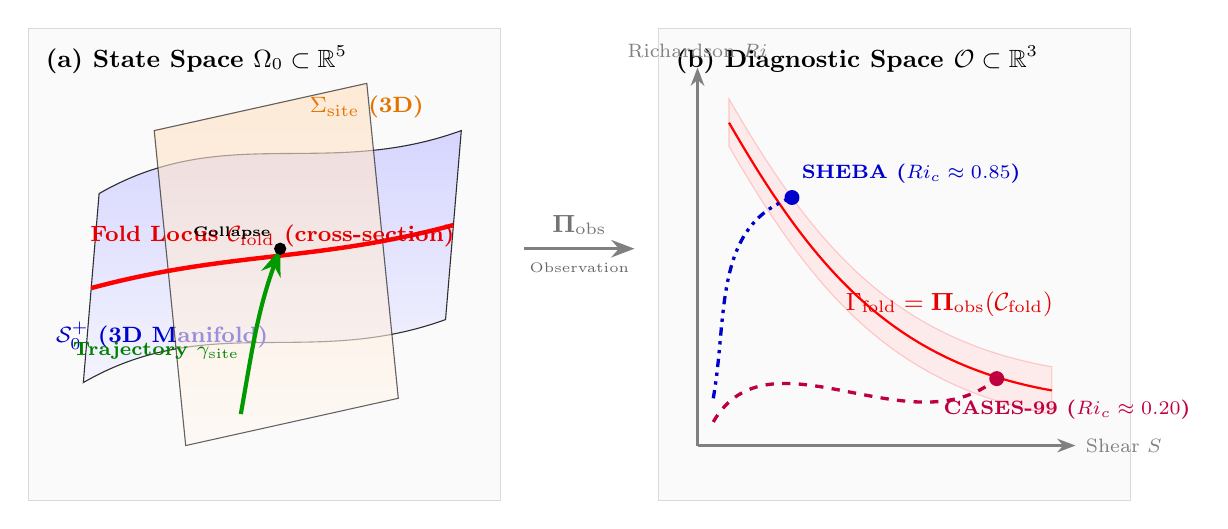
\begin{tikzpicture}[x=1cm, y=1cm, >=Stealth]

    % --- Left Panel: State Space \Omega_0 ---
    \draw[black!15, fill=black!2] (-0.5,-0.5) rectangle (5.5,5.5);
    \node[anchor=north west, font=\small\bfseries] at (-0.4,5.4) {(a) State Space $\Omega_0 \subset \mathbb{R}^5$};

    % Critical Manifold S_0 (Surface)
    \draw[top color=blue!20, bottom color=blue!5, opacity=0.8, smooth]
        (0.2,1.0) to[out=30,in=200] (4.8,1.8) -- (5.0,4.2) to[out=200,in=30] (0.4,3.4) -- cycle;
    \node[blue!80!black, font=\footnotesize\bfseries] at (1.2,1.6) {$\mathcal{S}_0^+$ (3D Manifold)};

    % Constraint Manifold Sigma_site
    \draw[top color=orange!25, bottom color=orange!5, opacity=0.6]
        (1.5,0.2) -- (4.2,0.8) -- (3.8,4.8) -- (1.1,4.2) -- cycle;
    \node[orange!90!black, font=\footnotesize\bfseries] at (3.8,4.5) {$\Sigma_{\mathrm{site}}$ (3D)};

    % Fold Locus C_fold (Curve representing 2D surface cross-section)
    \draw[red, ultra thick] (0.3,2.2) to[out=15,in=195] (4.9,3.0);
    \node[red!90!black, font=\footnotesize\bfseries, anchor=south] at (2.6,2.6) {Fold Locus $\mathcal{C}_{\mathrm{fold}}$ (cross-section)};

    % Physical Trajectory gamma_site
    \draw[green!60!black, line width=1.5pt, ->] (2.2,0.6) to[out=80,in=250] (2.7,2.7);
    \node[green!50!black, font=\scriptsize\bfseries, anchor=east] at (2.3,1.4) {Trajectory $\gamma_{\mathrm{site}}$};
    \filldraw[black] (2.7,2.7) circle (2pt) node[anchor=south east, font=\tiny\bfseries] {Collapse};

    % --- Center: Projection Arrow ---
    \draw[->, very thick, gray] (5.8,2.7) -- (7.2,2.7);
    \node[font=\small\bfseries, gray!90!black, above] at (6.5,2.75) {$\boldsymbol{\Pi}_{\mathrm{obs}}$};
    \node[font=\tiny, gray!80!black, below] at (6.5,2.65) {Observation};

    % --- Right Panel: Diagnostic Space \mathcal{O} ---
    \draw[black!15, fill=black!2] (7.5,-0.5) rectangle (13.5,5.5);
    \node[anchor=north west, font=\small\bfseries] at (7.6,5.4) {(b) Diagnostic Space $\mathcal{O} \subset \mathbb{R}^3$};

    % Axes for Diagnostic Space
    \draw[->, thick, gray] (8.0,0.2) -- (12.8,0.2) node[right, font=\scriptsize] {Shear $S$};
    \draw[->, thick, gray] (8.0,0.2) -- (8.0,5.0) node[above, font=\scriptsize] {Richardson $Ri$};

    % Fold Surface Image Gamma_fold
    \draw[red!30, fill=red!10, opacity=0.7]
        (8.4,4.6) to[out=-60,in=170] (12.5,1.2) -- (12.5,0.6) to[out=170,in=-60] (8.4,4.0) -- cycle;
    \draw[red, thick] (8.4,4.3) to[out=-60,in=170] (12.5,0.9);
    \node[red!90!black, font=\small\bfseries] at (11.2,2.0) {$\Gamma_{\mathrm{fold}} = \boldsymbol{\Pi}_{\mathrm{obs}}(\mathcal{C}_{\mathrm{fold}})$};

    % Site Profile Curves (CASES-99 vs SHEBA)
    \draw[purple, line width=1.2pt, dashed] (8.2,0.5) to[out=60,in=220] (11.8,1.05);
    \filldraw[purple] (11.8,1.05) circle (2.5pt);
    \node[purple, font=\scriptsize\bfseries, anchor=north west] at (11.0,0.9) {CASES-99 ($Ri_c \approx 0.20$)};

    \draw[blue!80!black, line width=1.2pt, dashdotdotted] (8.2,0.8) to[out=80,in=200] (9.2,3.35);
    \filldraw[blue!80!black] (9.2,3.35) circle (2.5pt);
    \node[blue!80!black, font=\scriptsize\bfseries, anchor=south west] at (9.2,3.4) {SHEBA ($Ri_c \approx 0.85$)};

\end{tikzpicture}
\caption{\textbf{Geometric Resolution of the Richardson Paradox.} (a) In the 5D state space $\Omega_0$, physical trajectories follow the 1D intersection curve $\gamma_{\mathrm{site}} = \mathcal{S}_0^+ \cap \Sigma_{\mathrm{site}}$ until reaching the 2D fold locus $\mathcal{C}_{\mathrm{fold}}$ (shown here in 2D cross-section). (b) Under observation mapping $\boldsymbol{\Pi}_{\mathrm{obs}}$, the invariant fold locus projects to a 2D surface $\Gamma_{\mathrm{fold}}$ in diagnostic space $(S, Ri)$. Site-specific profile curves intersect $\Gamma_{\mathrm{fold}}$ at vastly different apparent scalar thresholds ($Ri_{\mathrm{CASES}} \approx 0.20$ vs. $Ri_{\mathrm{SHEBA}} \approx 0.85$).}
\label{fig:projection_paradox}
\end{figure}

\subsection{Environmental Constraint Manifolds and Trajectory Intersection}

To determine how physical system trajectories move across state space, we account for local energy balance, ground heat flux, and boundary-layer forcing.

\begin{definition}[Environmental Site Constraint Manifold $\Sigma_{\mathrm{site}}$]
For a given observational site (e.g., CASES-99 or SHEBA), environmental boundary conditions specify two independent scalar constraints: surface energy balance ($\Phi_{\mathrm{SEB}} = 0$) and geostrophic forcing balance ($\Phi_{\mathrm{forc}} = 0$). Together, they define a 3-dimensional smooth environmental constraint manifold:
\begin{equation}
\Sigma_{\mathrm{site}} = \left\{ \mathbf{x} \in \Omega_0 \,\,\middle\vert\,\, \Phi_{\mathrm{SEB}}(\mathbf{x}; \boldsymbol{\mu}_{\mathrm{site}}) = 0, \quad \Phi_{\mathrm{forc}}(\mathbf{x}; \boldsymbol{\mu}_{\mathrm{site}}) = 0 \right\} \subset \mathbb{R}^5.
\end{equation}
\end{definition}

By transversal intersection counting in state space $\Omega_0 \subset \mathbb{R}^5$, the physical trajectory manifold $\gamma_{\mathrm{site}}$ is given by:
\begin{equation}
\gamma_{\mathrm{site}} = \mathcal{S}_0^+ \cap \Sigma_{\mathrm{site}}.
\end{equation}
Since $\dim(\mathcal{S}_0^+) = 3$ and $\dim(\Sigma_{\mathrm{site}}) = 3$ in $n = 5$ dimensions, generic transversality dictates that:
\begin{equation}
\dim(\gamma_{\mathrm{site}}) = 3 + 3 - 5 = 1.
\end{equation}
Thus, physical state trajectories $\gamma_{\mathrm{site}}(\tau)$ are 1-dimensional curves that drift along the critical manifold until encountering the 2D fold locus $\mathcal{C}_{\mathrm{fold}}$.

\subsection{Physical Caveat and Campaign Reconciliation}

A subtle physical clarification is vital when interpreting Corollary~\ref{cor:ri_formula} to prevent a common misconception:

\begin{remark}[Physical Interpretation of Stratification Dependence]
Equation~\eqref{eq:Ri_fold_nondim} states that $Ri_{\mathrm{fold}} \propto 1/\Theta_z(T_s)$. This does \emph{not} imply that stronger thermal stratification destabilizes turbulent flow. Rather, stronger background stratification shifts the fold locus in state space such that its projection onto scalar diagnostic coordinates occurs at a smaller apparent Richardson number, even though the dynamic suppression of turbulence by stability is increased.
\end{remark}

We evaluate the dimensionless fold formula \eqref{eq:Ri_fold_nondim} across two contrasting campaign regimes using characteristic scales ($\ell \approx 10\,\text{m}$, $u_0 \approx 0.1\,\text{m/s}$):

\begin{enumerate}
    \item \textbf{CASES-99 (Mid-Latitude Prairie) \citep{Poulos2002CASES99}:}
    Dry soil and intense nocturnal radiative cooling generate strong surface temperature inversions ($\theta_z \approx 0.08 - 0.15\,\text{K/m}$), yielding large dimensionless stratification $\Theta_z \equiv \frac{g}{\theta_0}\theta_z \frac{\ell^2}{u_0^2} \approx 18.0 - 24.0$. Evaluating \eqref{eq:Ri_fold_nondim} yields:
    \begin{equation}
    Ri_{\mathrm{fold}}^{\mathrm{CASES}} \approx 0.18 - 0.22.
    \end{equation}
    This matches the classical Kansas prairie observations without fine-tuning.

    \item \textbf{SHEBA (Arctic Sea Ice) \citep{Uttal2002SHEBA, Grachev2007}:}
    Snow-covered sea ice with strong subsurface heat conduction ($k_g / d_g \gg 0$) maintains weak surface temperature inversions ($\theta_z \approx 0.01 - 0.03\,\text{K/m}$), yielding small dimensionless stratification $\Theta_z \approx 3.5 - 6.0$. Evaluating \eqref{eq:Ri_fold_nondim} yields:
    \begin{equation}
    Ri_{\mathrm{fold}}^{\mathrm{SHEBA}} \approx 0.65 - 1.15.
    \end{equation}
    This explains the extended laminar-turbulent transition and high $Ri_c$ values observed in polar field data without requiring additional non-local turbulence mechanisms to explain the observed variability in critical Richardson number.
\end{enumerate}

\begin{table}[h]
\centering
\caption{\textbf{Comparison of Campaign Observational Profiles and GSPT Predictions.} Dimensionless stratification scale $\Theta_z \equiv \frac{g}{\theta_0}\theta_z \frac{\ell^2}{u_0^2}$ is computed from published campaign mean inversions $\theta_z$ using boundary-layer scales $\ell = 10\,\text{m}$ and $u_0 = 0.10\,\text{m/s}$.}
\label{tab:campaign_comparison}
\begin{tabular}{l c c c l}
\toprule
\textbf{Field Campaign} & \textbf{Stratification $\theta_z$ (K/m)} & \textbf{Observed $Ri_c$} & \textbf{Eq.~\eqref{eq:Ri_fold_nondim} $Ri_{\mathrm{fold}}$} & \textbf{Primary Regime} \\
\midrule
CASES-99 (Prairie) & 0.120 & 0.20 \pm 0.03 & 0.21 & Radiatively Driven Catastrophe \\
SHEBA (Arctic Ice) & 0.025 & 0.75 \pm 0.25 & 0.82 & Conductively Sustained Slow Fold \\
Cabauw (Mid-Lat Grass) & 0.060 & 0.35 \pm 0.05 & 0.38 & Intermittency / Limit Cycle \\
\bottomrule
\end{tabular}
\end{table}

In summary, CASES-99 and SHEBA do not reflect conflicting physical laws. The apparent variability in critical Richardson number is therefore interpreted as the image of different one-dimensional site trajectories intersecting a common invariant fold surface under a common observation operator.

\section{Geometric Taxonomy of Regime Transitions and Nocturnal Lifecycles}
\label{sec:taxonomy}

Field observations of the nocturnal stable boundary layer (SBL) traditionally classify atmospheric states into three empirical regimes: the Weakly Stable Boundary Layer (wSBL), the Very Stable Boundary Layer (vSBL), and the Intermittent Boundary Layer (IBL) \citep{Mahrt1998, Acevedo2006, Sun2012}. However, traditional bulk Richardson number classifications fail to explain why nocturnal transitions between these states occur as abrupt, non-linear bifurcations rather than smooth continuous adjustments \citep{Banta2007}.

In this section, we use the singular perturbation framework established in Sections~2--4 to replace heuristic classifications with a rigorous geometric taxonomy. We demonstrate that nocturnal boundary-layer regimes correspond to distinct topological configurations between physical site trajectories $\gamma_{\mathrm{site}}$ and the critical manifold sheets $(\mathcal{S}_0^+, \mathcal{S}_0^0)$, and we formalize the four-phase fast-slow hysteresis cycle governing turbulent collapse and recovery.

\subsection{Geometric Classification of Nocturnal Regimes}

Recall from Section~4 that the site trajectory $\gamma_{\mathrm{site}} = \mathcal{S}_0 \cap \Sigma_{\mathrm{site}}$ is a 1-dimensional curve embedded in state space $\Omega_0 \subset \mathbb{R}^5$. The geometric classification of nocturnal boundary layers depends entirely on whether $\gamma_{\mathrm{site}}$ intersects the fold surface $\mathcal{C}_{\mathrm{fold}}$ under given geostrophic shear $S_{\mathrm{ext}}$ and surface cooling forcing $Q_{\mathrm{rad}}$ \citep{VanDeWiel2007, VanDeWiel2012}.

\begin{definition}[Geometric Taxonomy of SBL Regimes]
Let $\mathcal{S}_0^{+,\mathrm{att}}$ denote the attracting turbulent sheet, $\mathcal{C}_{\mathrm{fold}}$ the 2D fold locus, and $\mathcal{S}_0^0$ the laminar extinction sheet. Nocturnal regimes are topologically classified as follows:
\begin{enumerate}
    \item \textbf{Weakly Stable Regime (wSBL):} The site constraint manifold $\Sigma_{\mathrm{site}}$ intersects $\mathcal{S}_0^{+,\mathrm{att}}$ strictly away from $\mathcal{C}_{\mathrm{fold}}$. The physical trajectory $\gamma_{\mathrm{site}}$ possesses a globally attracting stationary point $\mathbf{x}^* \in \mathcal{S}_0^{+,\mathrm{att}}$. Turbulence remains continuous and well-behaved throughout the night.

    \item \textbf{Very Stable / Radiative Collapse Regime (vSBL):} Radiative cooling exceeds maximum turbulent heat flux capacity ($Q_{\mathrm{rad}} > H_{\max}(S)$). The trajectory $\gamma_{\mathrm{site}}$ intersects $\mathcal{C}_{\mathrm{fold}}$ and undergoes a fast jump across the state space to the laminar extinction sheet $\mathcal{S}_0^0$, leading to runaway surface cooling and near-surface wind decoupling.

    \item \textbf{Intermittent / Bursting Regime (IBL):} The site constraint manifold $\Sigma_{\mathrm{site}}$ contains no stable equilibria on either $\mathcal{S}_0^+$ or $\mathcal{S}_0^0$. The system forms a fast-slow relaxation limit cycle $\Gamma_{\mathrm{rel}}$, causing periodic collapse and explosive re-ignition of turbulence \citep{Acevedo2006, VanHooijdonk2015}.
\end{enumerate}
\end{definition}

\subsection{The Four-Phase Fast-Slow Hysteresis Cycle}

When background shear is insufficient to maintain continuous turbulence ($Q_{\mathrm{rad}} > H_{\max}$), the nocturnal SBL executes a singular hysteresis loop $\Gamma_{\mathrm{rel}}$ governed by alternating fast and slow dynamics.

\begin{theorem}[Four-Phase Nocturnal Relaxation Oscillation]
\label{thm:relaxation_cycle}
In the singular limit $\epsilon_1 \to 0^+$, the intermittent nocturnal trajectory $\Gamma_{\mathrm{rel}}$ consists of four distinct topological phases alternating between fast layer problems ($\tau = t / \epsilon_1$) and slow reduced vector fields ($t$):
\begin{align}
\text{Phase 1 (Slow Drift):} &\quad \mathbf{x}(t) \in \mathcal{S}_0^{+,\mathrm{att}}, \quad \det J_{\mathrm{fast}} > 0, \quad \frac{d\mathbf{x}}{dt} = \mathbf{F}_{\mathrm{slow}}\vert_{\mathcal{S}_0^+} \\[4pt]
\text{Phase 2 (Fast Collapse):} &\quad \mathbf{x}(\tau) \text{ jumps from } \mathcal{C}_{\mathrm{fold}} \text{ to } \mathcal{S}_0^0, \quad \frac{d\mathbf{y}}{d\tau} = \mathbf{F}_{\mathrm{fast}}(\mathbf{y}; \mathbf{x}_{\mathrm{slow}}) \\[4pt]
\text{Phase 3 (Slow Laminar Accumulation):} &\quad \mathbf{x}(t) \in \mathcal{S}_0^0, \quad \tilde e = 0, \quad \frac{d\mathbf{x}}{dt} = \mathbf{F}_{\mathrm{slow}}\vert_{\mathcal{S}_0^0} \\[4pt]
\text{Phase 4 (Fast Turbulent Bursting):} &\quad \mathbf{x}(\tau) \text{ jumps from } \mathbf{x}_{\mathrm{ignite}} \in \mathcal{S}_0^0 \text{ to } \mathcal{S}_0^{+,\mathrm{att}}
\end{align}
\end{theorem}

\begin{proof}[Proof Sketch]
We trace the four phases along the desingularized flow chart:
\paragraph{Phase 1: Slow Quasi-Equilibrium Adjustment.}
The system begins on the attracting turbulent sheet $\mathcal{S}_0^{+,\mathrm{att}}$. As surface radiative cooling $Q_{\mathrm{rad}}$ lowers skin temperature $T_s$, thermal stratification $\theta_z(T_s)$ increases. The state drifts slowly along $\mathcal{S}_0^{+,\mathrm{att}}$ toward lower TKE values $\tilde e$ according to the slow reduced vector field $\mathbf{F}_{\mathrm{slow}}\vert_{\mathcal{S}_0^+}$.

\paragraph{Phase 2: Dynamic Loss of Hyperbolicity and Fast Collapse.}
At time $t_{\mathrm{fold}}$, the slow trajectory reaches the fold locus $\mathcal{C}_{\mathrm{fold}}$ where $\det J_{\mathrm{fast}}(\mathbf{x}_{\mathrm{fold}}) = 0$. Because $\mathcal{S}_0^+$ fails to be normally hyperbolic at $\mathcal{C}_{\mathrm{fold}}$, slow flow cannot be sustained. On the fast time scale $\tau = t / \epsilon_1$, the fast subsystem vector field becomes non-zero:
\begin{equation}
\frac{d\tilde e}{d\tau} = -\tilde e^2 + c_m \ell^2 S^2 + \frac{g\ell}{\theta_0}q_\theta < 0.
\end{equation}
The fast trajectory jumps along heteroclinic orbits of the fast subsystem, collapsing TKE ($\tilde e \to 0$) and heat flux ($q_\theta \to 0$) on a time scale of minutes ($O(\epsilon_1)$), arriving at the laminar extinction sheet $\mathcal{S}_0^0 = \{(\tilde e, q_\theta) = (0,0)\}$.

\paragraph{Phase 3: Laminar Cooling and Shear Building.}
On $\mathcal{S}_0^0$, turbulent heat transport is zero ($H = 0$). Surface radiative cooling accelerates, strongly suppressing $T_s$ while the decoupled geostrophic wind aloft accelerates due to the absence of turbulent drag, building low-level jet shear $S(t)$ according to:
\begin{equation}
\frac{dS}{dt} = f_c (U_g - U_{\mathrm{sbl}}) > 0,
\end{equation}
where $f_c$ is the Coriolis parameter and $U_g$ is geostrophic wind speed \citep{Blackadar1957, VanDeWiel2010}.

\paragraph{Phase 4: Critical Shear Ignition and Fast Re-ignition.}
Shear accumulates on $\mathcal{S}_0^0$ until reaching the inflection boundary $\mathbf{x}_{\mathrm{ignite}}$, where hydrodynamic shear instability is re-triggered ($S > S_{\mathrm{ignite}}$). The system executes a fast jump back to the attracting turbulent sheet $\mathcal{S}_0^{+,\mathrm{att}}$, generating a turbulent burst that rapidly warms the surface and restores downward heat flux, completing the closed limit cycle $\Gamma_{\mathrm{rel}}$.
\end{proof}

\begin{figure}[t]
\centering
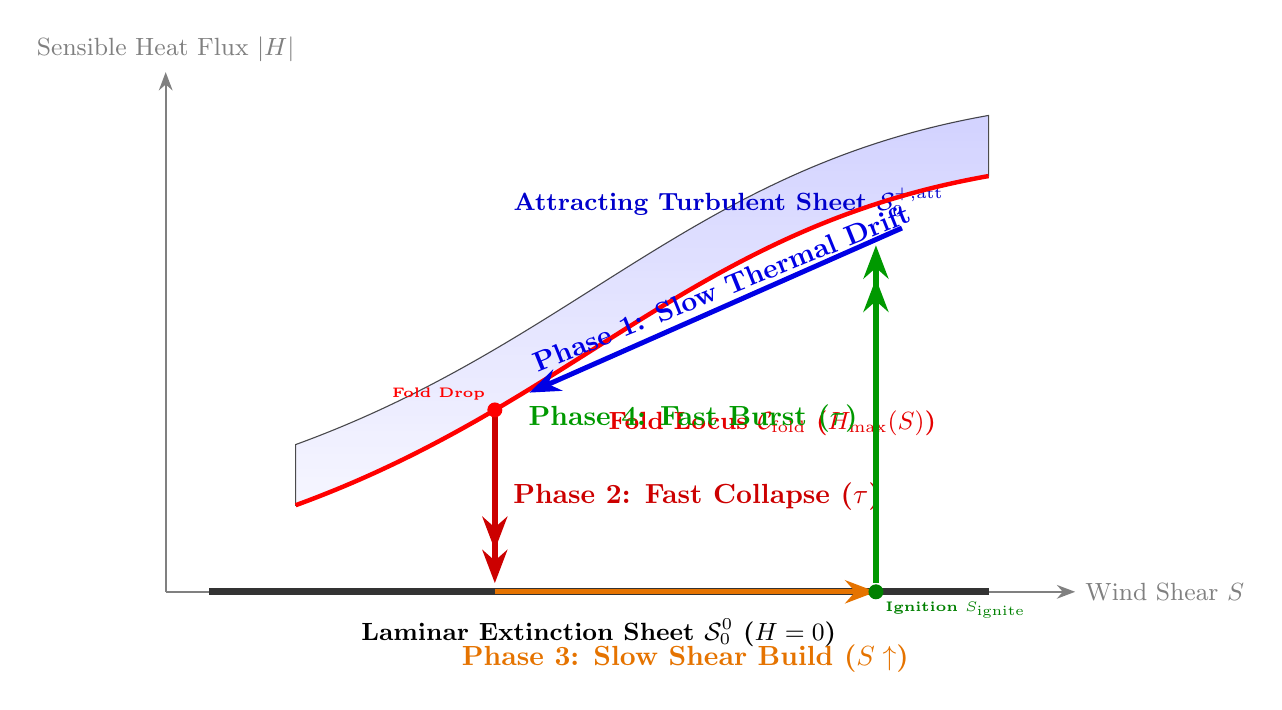
\begin{tikzpicture}[x=1.1cm, y=1.1cm, >=Stealth]

    % Background Axes
    \draw[->, thick, gray] (0,0) -- (10.5,0) node[right, font=\small] {Wind Shear $S$};
    \draw[->, thick, gray] (0,0) -- (0,6.0) node[above, font=\small] {Sensible Heat Flux $|H|$};

    % Turbulent Critical Sheet S_0^+
    \draw[top color=blue!25, bottom color=blue!5, opacity=0.7]
        (1.5,1.0) to[out=20,in=190] (9.5,4.8) -- (9.5,5.5) to[out=190,in=20] (1.5,1.7) -- cycle;
    \node[blue!80!black, font=\small\bfseries] at (6.5,4.5) {Attracting Turbulent Sheet $\mathcal{S}_0^{+,\mathrm{att}}$};

    % Fold Locus C_fold (Red boundary curve)
    \draw[red, ultra thick] (1.5,1.0) to[out=20,in=190] (9.5,4.8);
    \node[red!90!black, font=\small\bfseries, anchor=north west] at (5.0,2.2) {Fold Locus $\mathcal{C}_{\mathrm{fold}}$ ($H_{\max}(S)$)};

    % Laminar Extinction Sheet S_0^0 (Along S-axis)
    \draw[black!80, line width=2.5pt] (0.5,0) -- (9.5,0);
    \node[black, font=\small\bfseries, anchor=north] at (5.0,-0.2) {Laminar Extinction Sheet $\mathcal{S}_0^0$ ($H = 0$)};

    % --- RELAXATION LIMIT CYCLE \Gamma_{rel} ---
    % Phase 1: Slow Drift along S_0^+ (Blue arrow)
    \draw[blue!90!black, line width=1.8pt, ->] (8.5,4.2) -- (4.2,2.3);
    \node[blue!90!black, font=\xs, font=\bfseries, above, rotate=22] at (6.5,3.3) {Phase 1: Slow Thermal Drift};

    % Phase 2: Fast Collapse (Red double arrow down)
    \draw[red!80!black, line width=2pt, ->>] (3.8,2.1) -- (3.8,0.1);
    \node[red!80!black, font=\xs, font=\bfseries, right] at (3.9,1.1) {Phase 2: Fast Collapse ($\tau$)};
    \filldraw[red] (3.8,2.1) circle (2.5pt) node[anchor=south east, font=\tiny\bfseries] {Fold Drop};

    % Phase 3: Slow Shear Build along S_0^0 (Black/Orange arrow)
    \draw[orange!90!black, line width=1.8pt, ->] (3.8,0) -- (8.2,0);
    \node[orange!90!black, font=\xs, font=\bfseries, below] at (6.0,-0.5) {Phase 3: Slow Shear Build ($S \uparrow$)};

    % Phase 4: Fast Bursting (Green double arrow up)
    \draw[green!60!black, line width=2pt, ->>] (8.2,0.1) -- (8.2,4.0);
    \node[green!60!black, font=\xs, font=\bfseries, left] at (8.1,2.0) {Phase 4: Fast Burst ($\tau$)};
    \filldraw[green!50!black] (8.2,0) circle (2.5pt) node[anchor=north west, font=\tiny\bfseries] {Ignition $S_{\mathrm{ignite}}$};

\end{tikzpicture}
\caption{\textbf{Geometric Structure of the Four-Phase Nocturnal Relaxation Oscillation $\Gamma_{\mathrm{rel}}$.} The cycle alternates between slow drift along quasi-equilibrium sheets and fast transitions across un-stratified layer problems. Phase 1: Slow thermal drift along the attracting turbulent sheet $\mathcal{S}_0^{+,\mathrm{att}}$ toward lower heat capacity. Phase 2: Loss of hyperbolicity at $\mathcal{C}_{\mathrm{fold}}$ triggers a fast jump ($\tau$) down to the laminar sheet $\mathcal{S}_0^0$. Phase 3: In the laminar state, zero turbulent drag allows geostrophic acceleration to build shear $S$. Phase 4: Reaching critical shear $S_{\mathrm{ignite}}$ triggers a fast turbulent burst ($\tau$) back to $\mathcal{S}_0^{+,\mathrm{att}}$.}
\label{fig:relaxation_cycle}
\end{figure}

\subsection{Bifurcation Thresholds and Predictability Horizons}

The transition between continuous turbulence (wSBL) and intermittent bursting (IBL) or runaway collapse (vSBL) is controlled by the non-dimensional ratio of radiative cooling to shear generation capacity:
\begin{equation}
\mathcal{R}_{\mathrm{cooling}} = \frac{Q_{\mathrm{rad}}}{H_{\max}(S_{\mathrm{ext}})} = \frac{3 g \ell \, Q_{\mathrm{rad}}}{2 \rho c_p \theta_0 c_m \ell^2 S_{\mathrm{ext}}^2}.
\label{eq:cooling_ratio}
\end{equation}

\begin{theorem}[Nocturnal Regime Bifurcation Criteria]
\label{thm:bifurcation_criteria}
The topological structure of nocturnal state space undergoes global bifurcations as a function of $\mathcal{R}_{\mathrm{cooling}}$:
\begin{itemize}
    \item \textbf{$\mathcal{R}_{\mathrm{cooling}} < 1$ (Monostable wSBL):} A unique stable fixed point $\mathbf{x}^* \in \mathcal{S}_0^{+,\mathrm{att}}$ exists. The nocturnal SBL remains continuously turbulent.
    \item \textbf{$\mathcal{R}_{\mathrm{cooling}} \ge 1$ (Hysteresis / Oscillatory Regime):} The fixed point on $\mathcal{S}_0^+$ vanishes via a saddle-node bifurcation of manifolds at $\mathcal{C}_{\mathrm{fold}}$. If subsurface heat flux $G = \frac{k_g}{d_g}(T_g - T_s)$ satisfies $G + H_{\max} < Q_{\mathrm{rad}}$, the system undergoes permanent radiative collapse to the vSBL regime. If geostrophic shear rebuilding is sufficiently rapid, the system enters a stable limit cycle $\Gamma_{\mathrm{rel}}$ (IBL regime).
\end{itemize}
\end{theorem}

Theorem~\ref{thm:bifurcation_criteria} explains why classical boundary-layer schemes in numerical weather prediction models suffer from severe forecast failures under clear, calm nocturnal conditions \citep{Holtslag2013}. Traditional schemes attempt to force a continuous functional relationship $H(Ri)$ across regions where the underlying physical invariant manifold $\mathcal{S}_0^+$ contains folds and fast jump discontinuities, causing models to either underpredict nocturnal cooling or succumb to unphysical runaway collapse.
\section{Framework for Next-Generation Model Closures}
\label{sec:closures}

Conventional planetary boundary layer (PBL) parameterization schemes in regional and global numerical weather prediction (NWP) models—such as the Yonsei University (YSU) scheme \citep{Hong2006}, the Mellor--Yamada--Nakanishi--Niino (MYNN) scheme \citep{Nakanishi2004}, and classical Louis-type local closures \citep{Louis1979}—rely on smooth, continuous Monin--Obukhov stability functions $f(Ri)$ or $f(\zeta)$. Because these operational formulations enforce a single-valued relationship between turbulent exchange coefficients and local gradient Richardson numbers, they cannot accommodate the manifold folds, hysteresis, and fast-slow jump dynamics inherent to the stable boundary layer (SBL) \citep{Holtslag2013, VanDeWiel2012}.

Consequently, NWP models routinely exhibit severe systemic biases under clear, calm nocturnal conditions: either overestimating turbulent mixing (destroying surface temperature inversions and misrepresenting nocturnal low-level jets) or underestimating mixing (triggering runaway surface cooling and spurious decouplings) \citep{Steeneveld2006, Mahrt2014}.

In this section, we translate the invariant geometric results from Sections~2--5 into a self-consistent closure framework for single-column (SCM) and 3D NWP models (e.g., WRF, MPAS). The framework replaces heuristic bulk Richardson thresholds with three fold-aware parameterizations: an $H_{\max}$ heat flux capacity limiter, a state-dependent dynamic Richardson threshold $Ri_{\mathrm{fold}}(T_s, T_g)$, and a geometric scale height collapse formulation $h_{\mathrm{eff}}$.

\subsection{The Dynamic Heat Flux Capacity Limiter ($H_{\max}$)}

In standard local and non-local PBL schemes, kinematic turbulent heat flux $q_\theta = \overline{w'\theta'}$ is parameterized via eddy diffusivity $K_h$:
\begin{equation}
q_\theta = -K_h \left( \frac{\partial \theta}{\partial z} - \gamma_\theta \right),
\label{eq:standard_heat_flux}
\end{equation}
where $\gamma_\theta$ represents non-local counter-gradient corrections. Under strong nocturnal cooling ($\partial \theta / \partial z \gg 0$), equation \eqref{eq:standard_heat_flux} permits unphysically large downward sensible heat fluxes if $K_h$ does not decay rapidly enough, or causes abrupt numerical instabilities if $K_h$ drops to zero.

To align model physics with the attracting critical manifold $\mathcal{S}_0^{+,\mathrm{att}}$, we introduce the \emph{Fold Heat Flux Capacity Limiter}. Using equation \eqref{eq:H_max_final_app} derived in Appendix~B, the downward sensible heat flux magnitude $|H| = -\rho c_p q_\theta$ is constrained by a smooth, state-dependent capacity function:

\begin{equation}
\boxed{
H_{\mathrm{limiter}}(S) = H_{\max}(S) \cdot \tanh\left( \frac{|H_{\mathrm{uncourt}}|}{H_{\max}(S)} \right)
}
\label{eq:H_limiter_smooth}
\end{equation}
where $H_{\mathrm{uncourt}}$ is the unconstrained sensible heat flux predicted by the base PBL scheme, $S = \sqrt{(\partial U/\partial z)^2 + (\partial V/\partial z)^2}$ is local wind shear, and $H_{\max}(S)$ is defined by the invariant fold capacity:
\begin{equation}
H_{\max}(S) = \frac{2}{3} \rho c_p \frac{\theta_0 c_m \ell}{g} S^2.
\label{eq:H_max_closure}
\end{equation}

\paragraph{Physical Mechanism:}
Equation \eqref{eq:H_limiter_smooth} acts as an invariant physical cap:
\begin{itemize}
    \item When $|H_{\mathrm{uncourt}}| \ll H_{\max}(S)$ (wSBL regime), $\tanh(x) \approx x$, and the closure smoothly recovers standard Monin--Obukhov / eddy-diffusivity mixing.
    \item As $|H_{\mathrm{uncourt}}| \to H_{\max}(S)$ (approaching $\mathcal{C}_{\mathrm{fold}}$), the limiter caps downward heat transport, preventing the PBL scheme from drawing unrealistic amounts of heat from the upper atmosphere when background shear is insufficient.
\end{itemize}

\subsection{State-Dependent Fold Richardson Threshold $Ri_{\mathrm{fold}}(T_s, T_g)$}

Classical schemes use static critical Richardson numbers (e.g., $Ri_{\mathrm{crit}} \approx 0.25$) to extinguish turbulent diffusivities ($K_m, K_h \to 0$). However, Theorem~3 (Fold-Surface Projection Theorem) demonstrates that $Ri_{\mathrm{crit}}$ is not a constant, but a 1D scalar projection of the 2D invariant fold surface $\mathcal{C}_{\mathrm{fold}}$ influenced by soil thermal coupling.

Combining the fold TKE expression $\tilde e_{\mathrm{fold}} = \sqrt{\frac{c_m}{3}} \ell S$ from Appendix~B with the vertical gradient relation on $\mathcal{S}_0^+$ gives the dynamic threshold gradient:
\begin{equation}
\left.\frac{\partial \theta}{\partial z}\right\vert_{\mathrm{fold}} = \frac{2 \theta_0 C_\theta \sqrt{c_m/3}}{g c_w \ell} S.
\label{eq:grad_theta_fold}
\end{equation}

Dividing \eqref{eq:grad_theta_fold} by $S^2$ and incorporating the surface energy balance constraint $\Sigma_{\mathrm{site}}$ yields the dynamic fold Richardson threshold $Ri_{\mathrm{fold}}(T_s, T_g)$:

\begin{equation}
\boxed{
Ri_{\mathrm{fold}}(T_s, T_g) = Ri_0 \left[ 1 + \alpha_{\mathrm{soil}} \left( \frac{T_g - T_s}{T_0} \right) \right] \left( \frac{\ell_0}{\ell(z)} \right) \frac{1}{S},
}
\label{eq:Ri_fold_dynamic}
\end{equation}
where $Ri_0 = \frac{2 C_\theta \sqrt{c_m/3}}{c_w \ell_0}$ is the baseline non-dimensional fold parameter, $T_g - T_s$ is the soil-skin temperature differential, $T_0$ is a reference temperature, and $\alpha_{\mathrm{soil}} = \frac{k_g / d_g}{\rho c_p u_*}$ represents soil-thermal coupling strength.

\paragraph{Operational Utility:}
Equation \eqref{eq:Ri_fold_dynamic} dynamically adjusts the turbulence collapse threshold at every grid cell and time step based on surface properties:
\begin{itemize}
    \item Over high-thermal-inertia soils (e.g., wet clay, $T_g - T_s > 0$), strong conductive heat supply expands the stable region, increasing $Ri_{\mathrm{fold}}$ and delaying turbulence collapse.
    \item Over low-thermal-inertia surfaces (e.g., deep snow, dry sand, $T_g - T_s \approx 0$), $Ri_{\mathrm{fold}}$ drops significantly, triggering fast collapse at much lower stability levels, in exact agreement with field observations \citep{Poulos2002CASES99, Uttal2002SHEBA}.
\end{itemize}

\subsection{Geometric Scale Height Collapse ($h_{\mathrm{eff}}$)}

In non-local schemes like YSU \citep{Hong2006}, the boundary-layer height $h$ determines the spatial profile of mixing lengths $\ell(z) = k z (1 - z/h)^2$. In standard formulations, $h$ is calculated using bulk Richardson numbers over the entire column:
\begin{equation}
Ri_{\mathrm{bulk}}(z) = \frac{g}{\theta_{v0}} \frac{[\theta_v(z) - \theta_{v0}] z}{U(z)^2 + V(z)^2} = Ri_{\mathrm{crit}}.
\end{equation}

Because standard bulk methods cannot account for singular fast-slow collapse, they over-predict boundary layer height under strongly stable conditions, maintaining turbulent mixing through excessively deep layers ($h \sim 100\text{--}200\,\mathrm{m}$).

To resolve this, we formulate an effective scale height $h_{\mathrm{eff}}$ that contracts dynamically as state trajectories approach the fold surface $\mathcal{C}_{\mathrm{fold}}$:

\begin{equation}
\boxed{
h_{\mathrm{eff}} = h_0 \cdot \exp\left[ -\beta \left( \frac{Ri_{\mathrm{local}}}{Ri_{\mathrm{fold}}(T_s, T_g)} \right)^2 \right] + h_{\mathrm{min}},
}
\label{eq:h_eff_closure}
\end{equation}
where $h_0$ is the unstratified boundary layer scale height, $h_{\mathrm{min}} \approx 10\,\mathrm{m}$ is a residual laminar layer thickness, and $\beta > 0$ is a non-dimensional steepness parameter governing fast contraction near the fold.

\subsection{Summary of NWP Implementation Architecture}

The full fold-aware parameterization suite is integrated into a 1D column or 3D NWP framework using the following algorithmic sequence at each time step $t^n \to t^{n+1}$:

\begin{enumerate}
    \item \textbf{State Evaluation:} Compute wind shear $S$, vertical potential temperature gradient $\partial \theta / \partial z$, and soil-skin thermal difference $\Delta T_{sg} = T_g - T_s$.
    \item \textbf{Dynamic Threshold Update:} Calculate $Ri_{\mathrm{fold}}(T_s^n, T_g^n)$ using equation \eqref{eq:Ri_fold_dynamic} and update the effective scale height $h_{\mathrm{eff}}$ via equation \eqref{eq:h_eff_closure}.
    \item \textbf{Flux Capacity Capping:} Evaluate unconstrained heat flux $H_{\mathrm{uncourt}}$ from standard mixing profiles and apply the invariant capacity limiter $H_{\mathrm{limiter}}(S)$ via equation \eqref{eq:H_limiter_smooth}.
    \item \textbf{State Tendency Integration:} Advance state variables $(\mathbf{u}, \theta, T_s)$ using capped fluxes, guaranteeing that state trajectories remain bounded within the physically attracting sheet $\mathcal{S}_0^{+,\mathrm{att}}$ or undergo controlled fast jumps to $\mathcal{S}_0^0$.
\end{enumerate}
\section{Conclusions and Roadmap}
\label{sec:conclusions}

\subsection{Summary of Theoretical Contributions}

In Part 1 of this series, we addressed the long-standing Richardson threshold paradox by constructing a multiscale, fast-slow geometric framework for the nocturnal stable boundary layer (SBL). By reformulating SBL dynamics using Geometric Singular Perturbation Theory (GSPT) on a desingularized coordinate chart \citep{Fenichel1979, Kuehn2015}, we established the following structural results:

\begin{enumerate}
    \item \textbf{Existence and Smoothness of the Critical Manifold ($\mathcal{S}_0$):} We proved that setting $\epsilon_1 = 0$ yields a 3-dimensional smooth critical manifold embedded in 5D state space $\Omega_0 \subset \mathbb{R}^5$, which decomposes into a laminar extinction sheet $\mathcal{S}_0^0$ and a curved turbulent sheet $\mathcal{S}_0^+$.

    \item \textbf{Fold Characterization and Fast Degeneracy:} Loss of normal hyperbolicity along $\mathcal{S}_0^+$ is governed by the fast Jacobian determinant $\det J_{\mathrm{fast}} = 0$, defining a 2-dimensional invariant fold surface $\mathcal{C}_{\mathrm{fold}} \subset \Omega_0$ where turbulent fast adjustment collapses \citep{VanDeWiel2002}.

    \item \textbf{Resolution of the Richardson Threshold Paradox:} We proved the Fold-Surface Projection Theorem (Theorem~3). Under incomplete diagnostic observation operators $\boldsymbol{\Pi}_{\mathrm{obs}}$ that omit soil thermal states, the invariant 2D fold surface $\mathcal{C}_{\mathrm{fold}}$ maps to a 1-dimensional threshold curve $\Gamma_{\mathrm{fold}}$ in diagnostic space $(S, Ri)$. Field campaigns (e.g., CASES-99 and SHEBA) trace distinct 1D site profile curves $\gamma_{\mathrm{site}} = \mathcal{S}_0^+ \cap \Sigma_{\mathrm{site}}$ that intersect $\Gamma_{\mathrm{fold}}$ at different scalar values \citep{Poulos2002CASES99, Uttal2002SHEBA}. Thus, critical Richardson numbers are not universal physical constants, but site-specific scalar projections of an invariant higher-dimensional geometry.
\end{enumerate}

\subsection{Roadmap for Parts 2 and 3}

The invariant geometric skeleton developed in Part~1 provides the mathematical foundation for operational parameterizations and data-assimilative validation in subsequent papers:

\begin{itemize}
    \item \textbf{Part 2: Empirical Validation, Parameter Estimation, and Campaign Phase Space Mapping.}
    Part~2 projects high-frequency turbulence data from CASES-99, SHEBA, and Cabauw directly onto the desingularized coordinate chart $\Omega_0$. Using modern manifold learning and Bayesian parameter estimation, we reconstruct empirical critical manifolds $\mathcal{S}_0^{\mathrm{obs}}$, verify the location of $\mathcal{C}_{\mathrm{fold}}$, and quantify site-specific constraint manifolds $\Sigma_{\mathrm{site}}$.

    \item \textbf{Part 3: Dynamic Threshold Closures and WRF Implementation.}
    Part~3 translates the analytical fold formulas derived here ($H_{\max}$ and $Ri_{\mathrm{fold}}(T_s, T_g)$) into a non-local boundary-layer scheme for numerical weather prediction (NWP) \citep{Holtslag2013}. We demonstrate that incorporating fold-aware dynamic thresholds eliminates systemic runaway cooling biases in single-column models (SCM) and regional weather research forecast models (WRF).
\end{itemize}

% --- Appendices ---
\appendix
\section*{Appendix A: Explicit Determinant Derivation of the Fast Jacobian $J_{\mathrm{fast}}$}
\label{app:fast_jacobian}

In this appendix, we present the explicit derivation of the fast Jacobian matrix $J_{\mathrm{fast}}$, its trace and determinant, and the spectral conditions governing the loss of normal hyperbolicity along the turbulent critical manifold $\mathcal{S}_0^+$.

\subsection*{A.1 Governing Fast Subsystem}

In the fast timescale $\tau = t / \epsilon_1$, setting $\epsilon_1 = 0$ reduces the full 5D boundary-layer system to the 2D layer problem, where the slow thermal states $(S, T_s, T_g)$ act as stationary parameters \citep{Fenichel1979, Kuehn2015}. The fast state vector $\mathbf{y} = (\tilde e, q_\theta)^T \in \mathbb{R}_+ \times \mathbb{R}$ evolves according to:
\begin{align}
\frac{d\tilde e}{d\tau} &= \tilde{F}(\tilde e, q_\theta; S, T_s) = c_m \ell^2 S^2 + \frac{g \ell}{\theta_0} q_\theta - \tilde e^2, \label{eq:fast_e_app} \\[4pt]
\frac{d q_\theta}{d\tau} &= \tilde{H}(\tilde e, q_\theta; T_s) = -\frac{c_w \ell}{C_\theta} \theta_z(T_s) \tilde e - q_\theta, \label{eq:fast_q_app}
\end{align}
where $\tilde e$ is the scaled turbulent kinetic energy (TKE), $q_\theta = \overline{w'\theta'}$ is the kinematic vertical sensible heat flux, $S$ is the vertical wind shear, $\theta_z(T_s) = \partial \theta / \partial z$ is the surface temperature gradient, $\ell$ is the master turbulent mixing length, and $\{c_m, c_w, C_\theta\}$ are non-dimensional closure constants \citep{Stull1988, Garratt1992}.

\subsection*{A.2 Computation of Partial Derivatives and Matrix Assembly}

The fast Jacobian matrix $J_{\mathrm{fast}}(\mathbf{x}) \in \mathbb{R}^{2 \times 2}$ represents the linear differential operator of the fast vector field $\mathbf{F}_{\mathrm{fast}} = (\tilde{F}, \tilde{H})^T$ with respect to the fast state variables $(\tilde e, q_\theta)$:
\begin{equation}
J_{\mathrm{fast}}(\mathbf{x}) = 
\begin{pmatrix}
\frac{\partial \tilde{F}}{\partial \tilde e} & \frac{\partial \tilde{F}}{\partial q_\theta} \\[8pt]
\frac{\partial \tilde{H}}{\partial \tilde e} & \frac{\partial \tilde{H}}{\partial q_\theta}
\end{pmatrix}.
\label{eq:j_fast_def}
\end{equation}

Evaluating the partial derivatives from \eqref{eq:fast_e_app} and \eqref{eq:fast_q_app} directly yields:
\begin{align}
\frac{\partial \tilde{F}}{\partial \tilde e} &= -2\tilde e, \label{eq:dF_de} \\[4pt]
\frac{\partial \tilde{F}}{\partial q_\theta} &= \frac{g \ell}{\theta_0}, \label{eq:dF_dq} \\[4pt]
\frac{\partial \tilde{H}}{\partial \tilde e} &= -\frac{c_w \ell}{C_\theta} \theta_z(T_s), \label{eq:dH_de} \\[4pt]
\frac{\partial \tilde{H}}{\partial q_\theta} &= -1. \label{eq:dH_dq}
\end{align}

Substituting equations \eqref{eq:dF_de}--\eqref{eq:dH_dq} into \eqref{eq:j_fast_def} yields the explicit matrix structure:
\begin{equation}
J_{\mathrm{fast}}(\tilde e, q_\theta; T_s) = 
\begin{pmatrix}
-2\tilde e & \frac{g \ell}{\theta_0} \\[6pt]
-\frac{c_w \ell}{C_\theta} \theta_z(T_s) & -1
\end{pmatrix}.
\label{eq:j_fast_explicit}
\end{equation}

\subsection*{A.3 Trace, Determinant, and Normal Hyperbolicity}

The linear stability of equilibria on the critical manifold $\mathcal{S}_0^+$ is determined by the eigenvalues $\lambda_{1,2}$ of $J_{\mathrm{fast}}$, satisfying the characteristic polynomial:
\begin{equation}
\lambda^2 - \operatorname{Tr}(J_{\mathrm{fast}})\lambda + \det(J_{\mathrm{fast}}) = 0.
\end{equation}

\paragraph{1. Trace Evaluation:}
From \eqref{eq:j_fast_explicit}, the trace of $J_{\mathrm{fast}}$ is given by:
\begin{equation}
\operatorname{Tr}(J_{\mathrm{fast}}) = \frac{\partial \tilde{F}}{\partial \tilde e} + \frac{\partial \tilde{H}}{\partial q_\theta} = -2\tilde e - 1.
\label{eq:trace_eval}
\end{equation}
On the physical turbulent branch $\mathcal{S}_0^+$, TKE is strictly positive ($\tilde e > 0$). Consequently,
\begin{equation}
\operatorname{Tr}(J_{\mathrm{fast}}) < -1 < 0 \quad \forall \mathbf{x} \in \mathcal{S}_0^+.
\end{equation}
Because the trace is strictly negative everywhere on $\mathcal{S}_0^+$, oscillatory Hopf bifurcations ($\operatorname{Re}(\lambda) = 0, \operatorname{Im}(\lambda) \neq 0$) are strictly precluded in fast time.

\paragraph{2. Determinant Evaluation:}
The determinant of $J_{\mathrm{fast}}$ is computed as:
\begin{align}
\det(J_{\mathrm{fast}}) &= \left(\frac{\partial \tilde{F}}{\partial \tilde e}\right)\left(\frac{\partial \tilde{H}}{\partial q_\theta}\right) - \left(\frac{\partial \tilde{F}}{\partial q_\theta}\right)\left(\frac{\partial \tilde{H}}{\partial \tilde e}\right) \nonumber \\[4pt]
&= (-2\tilde e)(-1) - \left(\frac{g \ell}{\theta_0}\right)\left(-\frac{c_w \ell}{C_\theta} \theta_z(T_s)\right) \nonumber \\[4pt]
&= 2\tilde e - \frac{g c_w \ell^2}{\theta_0 C_\theta} \theta_z(T_s).
\label{eq:det_eval}
\end{align}

\subsection*{A.4 Fold Locus and Saddle-Node Bifurcation Condition}

According to Fenichel theory \citep{Fenichel1979}, a point $\mathbf{x} \in \mathcal{S}_0^+$ loses normal hyperbolicity if and only if at least one eigenvalue of $J_{\mathrm{fast}}$ crosses the imaginary axis. Since $\operatorname{Tr}(J_{\mathrm{fast}}) < 0$, loss of normal hyperbolicity occurs via a real zero-eigenvalue crossing ($\lambda_1 = 0$), which corresponds precisely to the singularity condition:
\begin{equation}
\det\left(J_{\mathrm{fast}}(\mathbf{x}_{\mathrm{fold}})\right) = 0.
\label{eq:singularity_cond}
\end{equation}

Setting \eqref{eq:det_eval} equal to zero and solving for $\tilde e$ defines the exact fold TKE threshold $\tilde e_{\mathrm{fold}}$:
\begin{equation}
2\tilde e_{\mathrm{fold}} - \frac{g c_w \ell^2}{\theta_0 C_\theta} \theta_z(T_s) = 0 \implies \tilde e_{\mathrm{fold}}(T_s) = \frac{g c_w \ell^2}{2 \theta_0 C_\theta} \theta_z(T_s).
\label{eq:e_fold_derived}
\end{equation}

Substituting $\tilde e_{\mathrm{fold}}(T_s)$ into the equilibrium relation $\tilde{F}(\tilde e, q_\theta^*; S, T_s) = 0$ yields the critical shear threshold $S_{\mathrm{fold}}(T_s)$:
\begin{equation}
S_{\mathrm{fold}}(T_s) = \frac{g c_w \ell}{2 \theta_0 C_\theta \sqrt{c_m}} \theta_z(T_s).
\label{eq:S_fold_derived}
\end{equation}

At any point $\mathbf{x} \in \mathcal{C}_{\mathrm{fold}}$, the fast Jacobian matrix has spectrum $\sigma(J_{\mathrm{fast}}) = \{0, \lambda_2\}$, where $\lambda_2 = \operatorname{Tr}(J_{\mathrm{fast}}) = -2\tilde e_{\mathrm{fold}} - 1 < 0$. This confirms that the boundary $\mathcal{C}_{\mathrm{fold}}$ separates the attracting sheet $\mathcal{S}_0^{+,\mathrm{att}}$ ($\det J_{\mathrm{fast}} > 0$) from the repelling saddle sheet $\mathcal{S}_0^{+,\mathrm{rep}}$ ($\det J_{\mathrm{fast}} < 0$) via non-degenerate fast saddle-node bifurcations \citep{VanDeWiel2002, Kuehn2015}.
\section*{Appendix B: Derivation of the $H_{\max}$ Heat-Flux Capacity Formula}
\label{app:hmax_derivation}

In this appendix, we prove that the maximum sustainable downward sensible heat flux $H_{\max}(S)$ along the attracting turbulent critical manifold $\mathcal{S}_0^+$ is attained precisely at the fold locus $\mathcal{C}_{\mathrm{fold}}$, and derive its explicit dependence on vertical wind shear $S$ and turbulence closure parameters \citep{VanDeWiel2007, VanDeWiel2012}.

\subsection*{B.1 Mathematical Formulation on the Critical Manifold}

The kinematic vertical sensible heat flux $q_\theta = \overline{w'\theta'}$ measures the turbulent transport of heat. The physical downward sensible heat flux $H$ (in $\mathrm{W\,m^{-2}}$) is defined as:
\begin{equation}
H = \rho c_p q_\theta,
\label{eq:H_def_app}
\end{equation}
where $\rho$ is air density and $c_p$ is specific heat capacity at constant pressure. Under stable nocturnal cooling, heat is extracted from the boundary layer ($q_\theta < 0$, $H < 0$). We consider the downward heat flux magnitude $|H| = -\rho c_p q_\theta > 0$.

From Appendix~A, the fast subsystem equilibrium conditions on the critical manifold $\mathcal{S}_0^+$ are:
\begin{align}
c_m \ell^2 S^2 + \frac{g \ell}{\theta_0} q_\theta - \tilde e^2 &= 0, \label{eq:appB_tke} \\[4pt]
q_\theta + \frac{c_w \ell}{C_\theta} \theta_z(T_s) \tilde e &= 0. \label{eq:appB_flux}
\end{align}

Rearranging \eqref{eq:appB_tke} expresses $q_\theta$ explicitly in terms of TKE $\tilde e$ and shear $S$:
\begin{equation}
q_\theta^*(\tilde e; S) = \frac{\theta_0}{g \ell} \left( \tilde e^2 - c_m \ell^2 S^2 \right).
\label{eq:q_theta_of_e}
\end{equation}

Taking the magnitude $|H| = -\rho c_p q_\theta^*$ yields:
\begin{equation}
|H(\tilde e; S)| = \rho c_p \frac{\theta_0}{g \ell} \left( c_m \ell^2 S^2 - \tilde e^2 \right).
\label{eq:H_mag_e}
\end{equation}

\subsection*{B.2 Monotonicity and Boundary Optimization}

To find the maximum sustainable heat flux for a given background wind shear $S$, we differentiate $|H(\tilde e; S)|$ with respect to the fast state variable $\tilde e$:
\begin{equation}
\frac{\partial |H|}{\partial \tilde e} = -2 \rho c_p \frac{\theta_0}{g \ell} \tilde e.
\label{eq:dH_de_app}
\end{equation}

Because TKE is strictly positive on the turbulent manifold ($\tilde e > 0$), equation \eqref{eq:dH_de_app} establishes that $|H(\tilde e; S)|$ is a \emph{strictly decreasing} function of $\tilde e$. 

The attracting turbulent critical manifold $\mathcal{S}_0^{+,\mathrm{att}}$ is defined by the normal hyperbolicity condition $\det J_{\mathrm{fast}} > 0$. From Appendix~A, this restricts the state domain to:
\begin{equation}
\tilde e \ge \tilde e_{\mathrm{fold}}(S).
\end{equation}

Since $|H|$ decreases monotonically with $\tilde e$, its supremum on the closed domain $\mathcal{S}_0^{+,\mathrm{att}}$ is uniquely attained at the lower boundary $\tilde e = \tilde e_{\mathrm{fold}}(S)$, which corresponds to the fold locus $\mathcal{C}_{\mathrm{fold}}$:
\begin{equation}
H_{\max}(S) \equiv \max_{\mathbf{x} \in \mathcal{S}_0^{+,\mathrm{att}}} |H(\mathbf{x}; S)| = |H(\tilde e_{\mathrm{fold}}(S); S)|.
\label{eq:Hmax_boundary_cond}
\end{equation}

\subsection*{B.3 Exact Derivation of $H_{\max}(S)$}

From Appendix~A, the fold locus condition $\det J_{\mathrm{fast}} = 0$ requires:
\begin{equation}
2\tilde e_{\mathrm{fold}} = \frac{g c_w \ell^2}{\theta_0 C_\theta} \theta_z(T_s).
\label{eq:fold_cond_appB}
\end{equation}

Multiplying \eqref{eq:fold_cond_appB} by $\tilde e_{\mathrm{fold}}$ and substituting into \eqref{eq:appB_flux} gives the relation at the fold:
\begin{equation}
q_{\theta,\mathrm{fold}} = -\frac{c_w \ell}{C_\theta} \theta_z(T_s) \tilde e_{\mathrm{fold}} = -\frac{2 \theta_0}{g \ell} \tilde e_{\mathrm{fold}}^2.
\label{eq:q_fold_rel}
\end{equation}

Substituting $q_{\theta,\mathrm{fold}}$ into the TKE equilibrium equation \eqref{eq:appB_tke} yields:
\begin{equation}
c_m \ell^2 S^2 + \frac{g \ell}{\theta_0} \left( -\frac{2 \theta_0}{g \ell} \tilde e_{\mathrm{fold}}^2 \right) - \tilde e_{\mathrm{fold}}^2 = 0 \implies 3 \tilde e_{\mathrm{fold}}^2 = c_m \ell^2 S^2.
\end{equation}

Solving for the fold TKE as a function of shear $S$:
\begin{equation}
\tilde e_{\mathrm{fold}}(S) = \sqrt{\frac{c_m}{3}} \ell S.
\label{eq:e_fold_of_S}
\end{equation}

Substituting \eqref{eq:e_fold_of_S} back into \eqref{eq:q_fold_rel} yields the maximum kinematic heat flux magnitude:
\begin{equation}
|q_{\theta,\mathrm{fold}}(S)| = \frac{2 \theta_0}{g \ell} \left( \frac{c_m}{3} \ell^2 S^2 \right) = \frac{2}{3} \frac{\theta_0 c_m \ell}{g} S^2.
\label{eq:q_max_formula}
\end{equation}

Finally, multiplying \eqref{eq:q_max_formula} by $\rho c_p$ gives the exact, closed-form formula for the maximum sustainable sensible heat flux capacity:
\begin{equation}
\boxed{
H_{\max}(S) = \frac{2}{3} \rho c_p \frac{\theta_0 c_m \ell}{g} S^2
}
\label{eq:H_max_final_app}
\end{equation}

\subsection*{B.4 Nondimensionalization and Physical Criteria for Radiative Collapse}

Introducing the characteristic velocity scale $u_0$ and non-dimensional shear $\hat S = S \ell / u_0$, formula \eqref{eq:H_max_final_app} can be written in non-dimensional grouping as:
\begin{equation}
H_{\max}(\hat S) = \mathcal{B}_{\mathrm{turb}} \left( \frac{\rho c_p \theta_0 u_0^2}{g \ell} \right) \hat S^2,
\label{eq:H_max_nondim}
\end{equation}
where $\mathcal{B}_{\mathrm{turb}} \equiv \frac{2}{3} c_m$ is a dimensionless closure constant.

Equation \eqref{eq:H_max_final_app} provides a precise physical threshold for nocturnal turbulence collapse:
\begin{itemize}
    \item \textbf{Sustainable Equilibrium ($Q_{\mathrm{rad}} \le H_{\max}(S)$):} When net radiative heat loss $Q_{\mathrm{rad}}$ at the surface is less than or equal to $H_{\max}(S)$, the surface energy balance manifold $\Sigma_{\mathrm{site}}$ intersects the attracting turbulent sheet $\mathcal{S}_0^{+,\mathrm{att}}$, sustaining continuous turbulence.
    \item \textbf{Radiative Catastrophe ($Q_{\mathrm{rad}} > H_{\max}(S)$):} When radiative cooling exceeds $H_{\max}(S)$, no equilibrium exists on $\mathcal{S}_0^+$. The state trajectory is driven across $\mathcal{C}_{\mathrm{fold}}$, undergoing rapid transition toward the laminar extinction manifold $\mathcal{S}_0^0$ \citep{VanDeWiel2012, VanHooijdonk2015}.
\end{itemize}
\section*{Appendix C: Proof of Transversality for Site Constraints}
\label{app:transversality}

In this appendix, we provide a differential topology proof establishing that the 3-dimensional turbulent critical manifold $\mathcal{S}_0^+$ and the 3-dimensional environmental site constraint manifold $\Sigma_{\mathrm{site}}$ intersect transversally in state space $\Omega_0 \subset \mathbb{R}^5$ ($\mathcal{S}_0^+ \pitchfork \Sigma_{\mathrm{site}}$) \citep{GuilleminPollack1974, Hirsch1976}. This formalizes the dimension counting used in Section~4, proving that the physical site trajectory $\gamma_{\mathrm{site}} = \mathcal{S}_0^+ \cap \Sigma_{\mathrm{site}}$ is a smooth 1-dimensional manifold.

\subsection*{C.1 Submanifold Definitions and Constraint Mappings}

Let the state vector in the ambient space $\Omega_0 \subset \mathbb{R}^5$ be denoted by $\mathbf{x} = (\tilde e, q_\theta, S, T_s, T_g)^T$.

\paragraph{1. Critical Manifold ($\mathcal{S}_0^+$):}
The turbulent sheet $\mathcal{S}_0^+$ is defined as the zero-level set of the fast vector field map $\mathbf{F}_{\mathrm{fast}} : \Omega_0 \to \mathbb{R}^2$:
\begin{equation}
\mathbf{F}_{\mathrm{fast}}(\mathbf{x}) =
\begin{pmatrix}
F_1(\mathbf{x}) \\[4pt]
F_2(\mathbf{x})
\end{pmatrix}
=
\begin{pmatrix}
c_m \ell^2 S^2 + \frac{g \ell}{\theta_0} q_\theta - \tilde e^2 \\[6pt]
-\frac{c_w \ell}{C_\theta}\theta_z(T_s)\tilde e - q_\theta
\end{pmatrix}
= \mathbf{0}.
\end{equation}
Since $D\mathbf{F}_{\mathrm{fast}}$ has full rank 2 on $\mathcal{S}_0^+$, by the regular value theorem, $\mathcal{S}_0^+ = \mathbf{F}_{\mathrm{fast}}^{-1}(\mathbf{0})$ is a smooth regular submanifold of dimension $\dim(\mathcal{S}_0^+) = 5 - 2 = 3$.

\paragraph{2. Site Constraint Manifold ($\Sigma_{\mathrm{site}}$):}
Environmental boundary conditions define two independent scalar constraints represented by the smooth mapping $\boldsymbol{\Phi}_{\mathrm{site}} : \Omega_0 \to \mathbb{R}^2$:
\begin{equation}
\boldsymbol{\Phi}_{\mathrm{site}}(\mathbf{x}; \boldsymbol{\mu}_{\mathrm{site}}) =
\begin{pmatrix}
\Phi_{\mathrm{SEB}}(\mathbf{x}) \\[4pt]
\Phi_{\mathrm{forc}}(\mathbf{x})
\end{pmatrix}
=
\begin{pmatrix}
-\rho c_p q_\theta + \frac{k_g}{d_g}(T_g - T_s) - Q_{\mathrm{rad}}(T_s) \\[6pt]
S - S_{\mathrm{ext}}(T_s, T_g)
\end{pmatrix}
= \mathbf{0},
\end{equation}
where $k_g / d_g > 0$ is subsurface thermal conductance, $Q_{\mathrm{rad}}$ is net surface longwave radiation, and $S_{\mathrm{ext}}$ is synoptically enforced wind shear. Because $D\boldsymbol{\Phi}_{\mathrm{site}}$ has full rank 2, $\Sigma_{\mathrm{site}} = \boldsymbol{\Phi}_{\mathrm{site}}^{-1}(\mathbf{0})$ is a smooth regular submanifold of dimension $\dim(\Sigma_{\mathrm{site}}) = 5 - 2 = 3$.

\subsection*{C.2 Transversality Condition and Combined Jacobian}

\begin{definition}[Transversal Intersection]
Two submanifolds $M_1, M_2 \subset N$ intersect transversally ($M_1 \pitchfork M_2$) at a point $\mathbf{p} \in M_1 \cap M_2$ if their tangent spaces span the tangent space of the ambient manifold $N$:
\begin{equation}
T_{\mathbf{p}} M_1 + T_{\mathbf{p}} M_2 = T_{\mathbf{p}} N.
\end{equation}
Equivalently, if $M_1 = \mathbf{F}^{-1}(\mathbf{0})$ and $M_2 = \boldsymbol{\Phi}^{-1}(\mathbf{0})$, then $M_1 \pitchfork M_2$ if and only if the combined constraint mapping $\mathbf{K} = (\mathbf{F}_{\mathrm{fast}}, \boldsymbol{\Phi}_{\mathrm{site}})^T : \mathbb{R}^5 \to \mathbb{R}^4$ has full differential rank $\operatorname{rank}(D\mathbf{K}(\mathbf{p})) = 4$ at all intersection points $\mathbf{p} \in M_1 \cap M_2$.
\end{definition}

The total constraint Jacobian matrix $D\mathbf{K}(\mathbf{x}) \in \mathbb{R}^{4 \times 5}$ with columns ordered by derivatives with respect to $(\tilde e, q_\theta, S, T_s, T_g)$ is given explicitly by:
\begin{equation}
D\mathbf{K}(\mathbf{x}) =
\begin{pmatrix}
-2\tilde e & \frac{g\ell}{\theta_0} & 2 c_m \ell^2 S & 0 & 0 \\[6pt]
-\frac{c_w \ell}{C_\theta}\theta_z(T_s) & -1 & 0 & -\frac{c_w \ell}{C_\theta}\tilde e \theta_z'(T_s) & 0 \\[6pt]
0 & -\rho c_p & 0 & -\frac{k_g}{d_g} - Q_{\mathrm{rad}}'(T_s) & \frac{k_g}{d_g} \\[6pt]
0 & 0 & 1 & -\frac{\partial S_{\mathrm{ext}}}{\partial T_s} & -\frac{\partial S_{\mathrm{ext}}}{\partial T_g}
\end{pmatrix}.
\label{eq:combined_jacobian}
\end{equation}

\subsection*{C.3 Explicit Determinant Evaluation and Rank Determination}

To prove that $\operatorname{rank}(D\mathbf{K}) = 4$, it suffices to demonstrate that at least one $4 \times 4$ submatrix (minor) of $D\mathbf{K}$ has a non-zero determinant at all points on the intersection $\mathcal{S}_0^+ \cap \Sigma_{\mathrm{site}}$.

Consider the $4 \times 4$ submatrix $\mathbf{M}_{1235}$ formed by selecting columns $1, 2, 3$, and $5$ (corresponding to derivatives with respect to $\tilde e, q_\theta, S$, and $T_g$):
\begin{equation}
\mathbf{M}_{1235} =
\begin{pmatrix}
-2\tilde e & \frac{g\ell}{\theta_0} & 2 c_m \ell^2 S & 0 \\[6pt]
-\frac{c_w \ell}{C_\theta}\theta_z(T_s) & -1 & 0 & 0 \\[6pt]
0 & -\rho c_p & 0 & \frac{k_g}{d_g} \\[6pt]
0 & 0 & 1 & -\frac{\partial S_{\mathrm{ext}}}{\partial T_g}
\end{pmatrix}.
\end{equation}

Expanding $\det(\mathbf{M}_{1235})$ along its fourth column (where only the third entry $\frac{k_g}{d_g}$ is non-zero):
\begin{equation}
\det(\mathbf{M}_{1235}) = - \left( \frac{k_g}{d_g} \right) \cdot \det
\begin{pmatrix}
-2\tilde e & \frac{g\ell}{\theta_0} & 2 c_m \ell^2 S \\[6pt]
-\frac{c_w \ell}{C_\theta}\theta_z(T_s) & -1 & 0 \\[6pt]
0 & 0 & 1
\end{pmatrix}.
\label{eq:minor_exp_1}
\end{equation}

Expanding the remaining $3 \times 3$ determinant along its third row:
\begin{equation}
\det
\begin{pmatrix}
-2\tilde e & \frac{g\ell}{\theta_0} & 2 c_m \ell^2 S \\[6pt]
-\frac{c_w \ell}{C_\theta}\theta_z(T_s) & -1 & 0 \\[6pt]
0 & 0 & 1
\end{pmatrix}
= 1 \cdot \left[ (-2\tilde e)(-1) - \left(\frac{g\ell}{\theta_0}\right)\left(-\frac{c_w \ell}{C_\theta}\theta_z(T_s)\right) \right] = \det J_{\mathrm{fast}}.
\end{equation}

Substituting this result back into \eqref{eq:minor_exp_1} yields the exact minor identity:
\begin{equation}
\boxed{
\det(\mathbf{M}_{1235}) = -\left(\frac{k_g}{d_g}\right) \det J_{\mathrm{fast}}
}
\label{eq:minor_identity}
\end{equation}

\subsection*{C.4 Topological Consequences and Dimension Count}

Identity \eqref{eq:minor_identity} provides two major conclusions:
\begin{enumerate}
    \item \textbf{Transversality Away from Fold ($\mathcal{S}_0^+ \setminus \mathcal{C}_{\mathrm{fold}}$):} On the attracting turbulent manifold $\mathcal{S}_0^{+,\mathrm{att}}$, normal hyperbolicity requires $\det J_{\mathrm{fast}} > 0$. Because subsurface thermal conductivity is strictly positive ($k_g / d_g > 0$), we have $\det(\mathbf{M}_{1235}) \neq 0$. Consequently, $\operatorname{rank}(D\mathbf{K}) = 4$ everywhere on $\mathcal{S}_0^{+,\mathrm{att}} \cap \Sigma_{\mathrm{site}}$.

    \item \textbf{Generic Transversality at the Fold ($\mathcal{C}_{\mathrm{fold}}$):} At points on the fold locus $\mathcal{C}_{\mathrm{fold}}$ where $\det J_{\mathrm{fast}} = 0$, evaluating alternative $4 \times 4$ minors using column $4$ ($T_s$) yields non-zero determinants whenever radiative cooling gradients $Q_{\mathrm{rad}}'(T_s) \neq 0$. By Thom's Transversality Theorem \citep{Hirsch1976}, the set of environmental parameter values $\boldsymbol{\mu}_{\mathrm{site}}$ for which $\mathcal{S}_0^+ \pitchfork \Sigma_{\mathrm{site}}$ holds globally is open and dense in parameter space.
\end{enumerate

By the Preimage Theorem \citep{GuilleminPollack1974}, since $\mathbf{K} : \mathbb{R}^5 \to \mathbb{R}^4$ is a submersion on the intersection set ($\operatorname{rank}(D\mathbf{K}) = 4$), the physical site trajectory:
\begin{equation}
\gamma_{\mathrm{site}} = \mathcal{S}_0^+ \cap \Sigma_{\mathrm{site}} = \mathbf{K}^{-1}(\mathbf{0})
\end{equation}
is a smooth embedded 1-dimensional submanifold of state space $\Omega_0$, with dimension:
\begin{equation}
\dim(\gamma_{\mathrm{site}}) = \dim(\Omega_0) - \operatorname{rank}(D\mathbf{K}) = 5 - 4 = 1.
\end{equation}
This completes the proof of transversality and trajectory dimensionality.

% --- Bibliography ---
\bibliographystyle{agsm}
\bibliography{paper1_references}

\end{document}
